\documentclass[12pt,twoside]{article}

\usepackage{svn-multi}
\svnidlong{$HeadURL: svn://glauber@ze.ic.unicamp.br/GlauberMSc/TechReport/TechReportMSc.tex $}{$LastChangedDate: 2009-09-26 12:37:42 -0300 (Sat, 26 Sep 2009) $}{$LastChangedRevision: 341 $}{$LastChangedBy: glauber $}
\svnid{$Id: TechReportMSc.tex 341 2009-09-26 15:37:42Z glauber $}

\usepackage{techrep-ic}
%%\usepackage[brazil]{babel}
\usepackage[english]{babel}

%%For PDFLaTeX
%%Do not use inputenc with xe(la)tex!
%% \usepackage[latin1]{inputenc}
%\usepackage[utf8]{inputenc}
%\usepackage[T1]{fontenc}
%\usepackage[pdftex, draft=false, colorlinks=true, breaklinks=true, bookmarks=true, pdftitle={Creating a HasCASL Library}, pdfauthor={G. M. Cabral and A. V. Moura}]{hyperref}
%\usepackage{hypcap}
%%Fonts
%%\usepackage{pslatex}
%%\usepackage{palatino}
%\usepackage{ae,aecompl}
%%END For PDFLaTeX

%%For XeLaTeX
\usepackage[xetex, draft=false, colorlinks=true, breaklinks=true, bookmarks=true, pdftitle={Creating a HasCASL Library}, pdfauthor={G. M. Cabral and A. V. Moura}]{hyperref}
\usepackage{hypcap}
%Fonts
\usepackage{fontspec} % provides font selecting commands 
\usepackage{xunicode} % provides unicode character macros 
\usepackage{xltxtra}  % provides some fixes/extras 
\defaultfontfeatures{Scale=MatchLowercase,Mapping=tex-text}
%For printing - few ink
%\setmainfont{Spranq Eco Sans}
%\setsansfont{Spranq Eco Sans}
%\setmonofont{Andale Mono}
%END For XeLaTeX

\usepackage{graphicx}
\usepackage{amsmath}

\usepackage{multicol}
\setlength{\columnseprule}{0.1pt}

%Bibliography
\usepackage{natbib}
\setcitestyle{numbers,square}
\bibliographystyle{plainnat}
%\bibliographystyle{abbrvnat}
%\bibliographystyle{unsrtnat}

\usepackage{url}

%For double line space
\usepackage{setspace}

%For Appendix
\usepackage{appendix}

%For Headers
\usepackage{fancyhdr}
\pagestyle{fancy}

%For Floats
\usepackage{float} 
\floatstyle{ruled}
%Spec float
\newfloat{spec}{htbp}{los}[section]
\floatname{spec}{Specification}
\numberwithin{spec}{subsection}
%Proof Excerpt float
\newfloat{proof}{htbp}{lop}[section]
\floatname{proof}{Isabelle Proof Script Excerpt}
\numberwithin{proof}{subsection}
%Proof Script float
\newfloat{pscript}{htbp}{lops}[section]
\floatname{pscript}{Isabelle Proof Script}
%\numberwithin{pscript}{subsection}
%Figures float
\newfloat{figure}{htbp}{pic}[section]
\floatname{figure}{Figure}
\numberwithin{figure}{subsection}
%Haskell source float
\newfloat{code}{htbp}{hs}[section]
\floatname{code}{Haskell Source Code}
\numberwithin{code}{subsection}

% My macros
% Macro for citing Appendix
\newcommand{\citeAppendix}[1][appendix:proofs]{Appendix~\ref{#1}, on page~\pageref{#1}}
%Macro for citing Specification
\newcommand{\citeSpec}[1]{Specification~\ref{#1}, on page~\pageref{#1}}
%Macro for citing Proof Excerpt
\newcommand{\citeProof}[1]{Isabelle Proof Script Excerpt~\ref{#1}, on page~\pageref{#1}}
%Macro for citing Full Proof Excerpt
\newcommand{\citePScript}[1]{Isabelle Proof Script~\ref{#1}, on page~\pageref{#1}}
%Macro for citing figure
\newcommand{\citeFig}[1]{Figure~\ref{#1}, on page~\pageref{#1}}
% Macro for referencing axiom
\newcommand{\axiom}[1]{{\tt \%(#1)\%}}
% Macro for referencing Haskell Code
\newcommand{\citeHaskell}[1]{Haskell Source Code~\ref{#1}, on page~\pageref{#1}}

\begin{document}

%%% PÁGINA DE CAPA %%%%%%%%%%%%%%%%%%%%%%%%%%%%%%%%%%%%%%%%%%%%%%%
% Número do relatório
\TRNumber{03}

% DATA DE PUBLICAÇÃO (PARA A CAPA)
\TRYear{09}  % Dois dígitos apenas
\TRMonth{01} % Numérico, 01-12

% LISTA DE AUTORES PARA CAPA (sem afiliações).
\TRAuthor{G. M. Cabral \and A. V. Moura}

% TÍTULO PARA A CAPA (use \\ para forçar quebras de linha).
\TRTitle{Creating a HasCASL Library}

\TRMakeCover

%%%%%%%%%%%%%%%%%%%%%%%%%%%%%%%%%%%%%%%%%%%%%%%%%%%%%%%%%%%%%%%%%%%%%%
% O que segue é apenas uma sugestão - sinta-se à vontade para
% usar seu formato predileto, desde que as margens tenham pelo
% menos 25mm nos quatro lados, e o tamanho do fonte seja pelo menos
% 11pt. Certifique-se também de que o título e lista de autores
% estão reproduzidos na íntegra na página 1, a primeira depois da
% página de capa.
%%%%%%%%%%%%%%%%%%%%%%%%%%%%%%%%%%%%%%%%%%%%%%%%%%%%%%%%%%%%%%%%%%%%%%

%%%%%%%%%%%%%%%%%%%%%%%%%%%%%%%%%%%%%%%%%%%%%%%%%%%%%%%%%%%%%%%%%%%%%%
% Nomes de autores ABREVIADOS e titulo ABREVIADO,
% para cabeçalhos em cada página.
%
%\markboth{Cabral e Moura}{A HasCASL Library}
%\pagestyle{myheadings}

\fancyhead{}
\fancyhead[el]{\thepage}
\fancyhead[er]{\textit{Cabral} e \textit{Moura}}
\fancyhead[ol]{\textit{A HasCASL Library}}
\fancyhead[or]{\thepage}
\fancyfoot{}
%\fancyfoot[l]{Rev: \svnrev\ (\svnfilerev)}
%\fancyfoot[r]{\svnyear-\svnmonth-\svnday \hspace{0.5cm} \svnhour:\svnminute} % Date
\renewcommand{\headrulewidth}{0pt}
\renewcommand{\footrulewidth}{0pt}

% Fancy style for chapter page (\maketitle uses plain style):
\fancypagestyle{plain}{%
\fancyhf{}
%\fancyfoot[ol]{Rev: \svnrev\ (\svnfilerev)}
\fancyfoot[oc]{\thepage}
%\fancyfoot[or]{\svnyear-\svnmonth-\svnday \hspace{0.5cm} \svnhour:\svnminute} % Date
\renewcommand{\headrulewidth}{0pt}
\renewcommand{\footrulewidth}{0pt}
}

%%%%%%%%%%%%%%%%%%%%%%%%%%%%%%%%%%%%%%%%%%%%%%%%%%%%%%%%%%%%%%%%%%%%%%
% TÍTULO e NOMES DOS AUTORES, completos, para a página 1.
% Use "\\" para quebrar linhas, "\and" para separar autores.
%
\title{Creating a HasCASL Library}

\author{Glauber Módolo Cabral\thanks{Instituto  de Computação, Universidade Estadual  de Campinas, 13081-970  Campinas,  SP.  Suporte CNPq Processo: 132039/2007-9}\and Arnaldo Vieira Moura\thanks{Instituto  de Computação, Universidade Estadual  de Campinas, 13081-970  Campinas,  SP. Suporte CNPq Processo: 305781/2005-7}}

\date{}

\maketitle

%%%%%%%%%%%%%%%%%%%%%%%%%%%%%%%%%%%%%%%%%%%%%%%%%%%%%%%%%%%%%%%%%%%%%%

%Configuring line spaces just for the text!
%\onehalfspacing
%\doublespacing

%%%%%%%%%%%%%%%%%%%%%%%%%%%%%%%%%%%%%%%%%%%%%%%%%%%%%%%%%%%%%%%%%%%%%%

\begin{abstract}
The effective use of a specification language depends on the availability of predefined specifications. Although the \textit{CASL} specification has such a library, that is not the case of the \textit{HasCASL} language, one of the \textit{CASL}'s extensions. Here we start to  specify such a library to the \textit{HasCASL} language, based on the Prelude library of the \textit{Haskell} programming language. When completed this approach would create a library that, after refinements, should lead to reusable specifications for real \textit{Haskell} programs. This technical report discusses the specification and verification of a kernel library to the \textit{HasCASL} language.
\end{abstract}

\section{Introduction}
In this report we show how to specify a library in the \textit{HasCASL} specification language. The intent it for this library to reuse previous specifications, as much as possible.

The practical use of a specification language requires that a default library exists. This could be a small library, used to guide new specifications, or, preferably, a predefined library that could be imported to construct other, larger, specifications.

The \textit{HasCASL} specification language does not yet have such a library. The \textit{CASL} specification language, of which \textit{HasCASL} is an extension, already has a default library with lots of specifications covering topics from simple data types to complex algebraic structures.

Here, we show how to construct a default library for the \textit{HasCASL} language based on the \textit{Prelude} library, from the \textit{Haskell} programming language. We describe the specification and the verification of our library. We include proofs and comments about the difficulties we faced.

This report is organized as follows. 
Section~\ref{Languages} introduces the languages involved in this work and details our proposal.
Section~\ref{Specification} describes our specifications, including their codes.
Section~\ref{Parsing} addresses the parsing and verification of the specifications.
Section~\ref{Discussion} discusses some problems we faced during the specification of the library.
Section~\ref{RelatedFrameworks} comments on some related specification languages.
Section~\ref{FutureWorks} lists open questions and topics for future work.
Section~\ref{Conclusions} concludes the report.
Appendix~\ref{appendix:proofs} lists the proof scripts used to verify the specifications.

\section{Languages}\label{Languages}
This section introduces the languages involved in our work. We start with a presentation of the \textit{CASL} specification language, briefly describing its syntax and semantic. Next, we introduce the \textit{Haskell} programming language, including some interesting concepts that we had to deal latter in specification. Next, we describe the \textit{HasCASL} specification language, a \textit{CASL} extension, which we used to write our specifications. We presented some main concepts of \textit{HasCASL} and a small example. Latter, we introduce the \textit{HasCASL} extension to the \textit{CASL} language and its related tool, namely \textit{Hets}, which is responsible for parsing and translating our specifications to be used with the theorem prover. Next, we introduce the \textit{Isabelle} theorem prover with a brief presentation of its main features. Finally, we describe our proposal for this work.

%Definir o nome correto da biblioteca \textit{CASL} e dizer que será referida como \textit{CASL} library.

\subsection{CASL}
The \textit{Common Algebraic Specification Language} (\textit{CASL}) emerged as the product of an international initiative to create an unified language for algebraic specifications containing  the largest possible set of known language constructions. This section describes the \textit{CASL} language \citep{Astesiano2002}.

With few exceptions, the characteristics of \textit{CASL} are present in some form or another in other specification languages. However, no previous single language had all the desired characteristics. Some sophisticated features require specific programming paradigms. On the other hand, methods for prototyping and specification generation work only in the absence of certain characteristics. For example, term rewriting requires specifications with equational or conditional equational axioms.

\textit{CASL} was constructed to be the kernel of a family of languages. Sub-languages are obtained through syntactic or semantic restrictions, while extensions are created to support the various programming paradigms. The language definition took into account previously planned extensions, such as the support to second order functions. \textit{CASL} is divided into several parts that can be understood and used separately, namely: 
\begin{itemize} 
\item Basic Specifications: contain declarations (of types and operations), definitions (of operations) and axioms (related operations); 
\item Structured Specifications: allow Basic Specifications to be combined in larger specifications; 
\item Architectural Specifications: define how specifications should be separated in an implementation, allowing reuse of specifications with dependence relations;
\item Specification libraries: similar specifications are joined together in these libraries; their syntax has facilities that allow version control and library distribution over the Internet.
\end{itemize}

Structured Specification language constructions are independent of the Basic Specifications. So, \textit{CASL} sub-languages or extensions can be created by extending or restricting Basic Specification language constructions, without the need to change any of the other three language parts. We now briefly describe the most important Basic Specification language constructions.

Basic Specification denotes a class of models which are many-sorted partial first order structures, i.e., many-sorted algebras with total and partial functions and predicates. These models are classified by signatures, which contain sort names, total and partial function names, predicate names and definitions (or profiles) for functions and predicates.

Specifications contain: declarations, which introduce components of the signature (operations or functions, and predicates), and axioms, which define properties of the structures that should be models of the specification. Operations may be declared total (by using `\verb.->.') or partial (by using `\verb.->?.'), and we can assign to this operations some common properties, such as associativity, avoiding the need for axiomatizing those properties for each different operation.

Partial operations are a simple way to treat errors (such as dividing by zero) and these errors are propagated to callers directly. When an argument of an operation is not defined, the operation result is also not defined. The errors and exceptions can be treated by super-types and sub-types. The domain of a partial function can be defined as a sub-type of that function's argument type in order to make this partial function a total function over the sub-type. Functions can be declared total rather than making them total by axioms.

Predicates are similar to operations but have no return type; only parameter types are declared. Predicates may be declared and defined at the same time, instead of having their declarations and axioms in separate sections.

Axioms are written as atomic first-order formulas. Variables used in axioms may be declared in three different ways: globally, before axiom declarations; locally to a list of formulas; or individually for each formula, using explicit quantification.

Formulas are interpreted in two-valued first order logic (with values true and false). Definedness assertions are used to indicate when a term is defined or not defined. Assertions may be declared explicitly by a keyword or implicitly by means of an existential equation. An existential equation, declared by using `\verb.=e=.' between two terms of the same type, is valid when both terms are defined and are equal. In contrast, strong equations, declared by using `\verb.=.' between terms, are also valid when both terms are undefined.

Sub-sort membership, indicated by `\verb.in.', creates a predicate asserting the membership of an element to a sort. It's a good practice to use existential equations when defining properties and strong equations when defining partial functions inductively.

\textit{CASL} uses a loose semantic for Basic Specifications, i.e., all structures that meet the axioms are selected as models. This semantic is interesting during requirement analysis because it creates very restrictive specifications that may be refined later by other axioms.

A data type can be declared as free, changing its loose semantic into an initial semantic. Thus, values of the same type that differ only in the order of the type constructor application are treated as different elements of that type.

The third semantic allowed in \textit{CASL} forces data types to be generated only by type constructor applications. This eliminates the confusion between terms, i.e., unless axioms force a term equality, all the terms of that type are different from each other. When needed, axioms can be used to reintroduce term equality.

Linear visibility is used to control term declaration except for type declarations, i.e., except in type declarations a term must be declared before its use.

\subsection{Haskell}
This section presents some general elements of the \textit{Haskell} programming language. Information provided here as well as further concepts can be found online \citep{learnHaskell} or in books \citep{Thompson1999}.

\textit{Haskell} is a pure, strong typed functional programming language with lazy evaluation. It resulted from the need of standardization in the domain of functional languages. The language is functional because it implements concepts of the $\lambda-Calculus$. So, the programming is done through function and computation applications. The language is strongly typed, i.e., the types of functions and values must be explicitly defined at compile time; otherwise, the compiler will try to bind those types to the broadest possible ones in the current context.
% Commenting on the disappearance of the concept of sequencing operations

Concepts of lazy evaluation and strict evaluation relate to the interpretation of the parameters of a function. Languages with strict evaluation calculates all parameters of a function call before running its body. In the case of languages with lazy evaluation, such as \textit{Haskell}, parameters of a function are evaluated only when they become necessary inside the function body.

The language is called purely functional because it does not allow a function application to change the global state of the program. Only changes to variables and values local to the function execution are allowed. Changing the global state of the program is a kind of side effect which is common in imperative languages. Functional programming languages that allow side effects are called non-pure.

To allow operations that may cause side effects to be executed without causing side effects to the whole program, \textit{Haskell} performs side-effect actions through a mathematical entity called a monad. Monads can sequence side-effect computations passing a copy of the actual global state implicitly to those computations. They prevent the side effects to change the real global state of the program.

\textit{Haskell} functions can be declared just as in the $\lambda-Calculus$ using \textit{Lambda Abstractions}, or the \textit{Haskell} syntax can be used. In both styles we can name function definitions for later reuse. If a function type is not defined, the compiler will compute the broader type in the corresponding context. The \textit{Haskell} syntax is preferred because it's easier and more practical for writing larger programs. Here, we show the function \verb.add. for summing two numbers, defined both using \textit{Lambda Abstractions} and in the \textit{Haskell} syntax, respectively. The compiler will append the type \verb.Integer -> Integer. to the functions, as we haven't declared their type:
\begin{verbatim}
add     = \x y -> x+y
add x y = x+y
\end{verbatim}

It is necessary to differentiate functions, such as the previously defined function \verb.add., from operators, such as the \verb.+. operator. A function in Haskell is always defined in a prefix way, while an operator uses infix definition. Besides these differences, it's possible to simulate a function with an operator and vice versa. Operators can be used as functions if enclosed in parenthesis; a function can be used as an operator if enclosed by back-quotes. We can use the operator \verb.+. as a function like this: \verb.(+) x y. and the function \verb.add. as an operator like this: \verb. x `add` y.

Just as in other functional languages, the main data represented in \textit{Haskell} are lists. There can be lists of primitive types, lists of tuples, lists of lists, lists of functions, etc.. The only requirement is that all elements of the list have the same type. The order and the quantity of elements within a list are taken into account when comparing them for equality.

Two basic operators to manipulate lists are ``\verb.:.'' (list construction) and ``\verb.++.'' (list concatenation). A list is always constructed from an empty list and some element, using the list construction operator. Two lists can be concatenated only if their elements have the same type.

Another feature largely explored in \textit{Haskell} programs is pattern matching. Functions can be defined by pattern matching their parameters, as follows:
\begin{verbatim}
fat :: Int -> Int
fat 1 = 1
fat x = x * fat(x-1)
\end{verbatim}

Each call to the function \verb.fat. will pattern match against each line of its definition,  from the first one to the last one, until the parameters of the function call match parameters from one of the definitions. Thus, the more specific definitions must come before the more generic ones. In the \citeHaskell{haskellcode}, we can see pattern matching applied in case expressions, list constructors and let expressions.

A fundamental tool in Haskell is the data type construction. A data type must have at least one constructor that may be empty or may have type variables. Type variables are used to construct polymorphic data types; the constructor and its type variables may be enclosed by parenthesis in order to avoid ambiguity. In the \citeHaskell{haskellcode}, we define the polymorphic type \verb.Split a b. with one constructor (\verb.Split b [[a]].). 

We can collect functions and data types from similar contexts into libraries. \textit{Haskell} libraries are called modules and can control which functions and data types from that module should be exposed to users. We've created a module in the \citeHaskell{haskellcode}, where all functions are exposed to the users. There is a standard \textit{Haskell} library, called \textit{Prelude}, which defines basic functions that operate on primitive types, such as \textit{Bool}, \textit{Char}, \textit{List} and \textit{String}. Also, there are numeric types and tuples involving those types. All \textit{Haskell} compilers must implement the \textit{Prelude} library ,as this implementation is part for the language definition.

\begin{code}\capstart
\footnotesize
\begin{verbatim}
module GenSort where
import Data.List
data Split a b = Split b [[a]]
genSort :: Ord a => ([a] -> Split a b) -> (Split a b -> [a]) -> [a] -> [a]
genSort split join l = case l of
  _ : _ : _ -> let Split c ls = split l in
               join $ Split c $ map (genSort split join) ls
  _ -> l
splitInsertionSort :: [a] -> Split a a
splitInsertionSort (a : l) = Split a [l]
joinInsertionSort :: Ord a => Split a a -> [a]
joinInsertionSort (Split a [l]) = insert a l
insertionSort :: Ord a => [a] -> [a]
insertionSort = genSort splitInsertionSort joinInsertionSort
splitQuickSort :: Ord a => [a] -> Split a a
splitQuickSort (a : l) =
  let (ls, gs) = partition (< a) l in Split a [ls, gs]
joinQuickSort :: Split a a -> [a]
joinQuickSort (Split a [ls, gs]) = ls ++ (a : gs)
quickSort :: Ord a => [a] -> [a]
quickSort = genSort splitQuickSort joinQuickSort
splitMergeSort :: [a] -> Split a ()
splitMergeSort l =
  let (l1, l2) = splitAt (div (length l) 2) l in Split () [l1, l2]
joinMergeSort :: Ord a => Split a () -> [a]
joinMergeSort (Split _ [l1, l2]) = merge l1 l2
merge :: Ord a => [a] -> [a] -> [a]
merge l1 l2 = case l1 of
  [] -> l2
  x1 : r1 -> case l2 of
     [] -> l1
     x2 : r2 -> if x1 < x2
       then x1 : merge r1 l2
       else x2 : merge l1 r2
mergeSort :: Ord a => [a] -> [a]
mergeSort = genSort splitMergeSort joinMergeSort
splitSelectionSort :: Ord a => [a] -> Split a a
splitSelectionSort l =
  let m = minimum l in Split m [delete m l]
joinSelectionSort :: Split a a -> [a]
joinSelectionSort (Split a [l]) = a : l
selectionSort :: Ord a => [a] -> [a]
selectionSort = genSort splitSelectionSort joinSelectionSort
\end{verbatim}
\caption{Haskell source code for GenSort sorting program}
\label{haskellcode}
\end{code}

\subsection{HasCASL}
This section presents the language \textit{HasCASL}\citep{SchroderMossakowski02}. The formal language definition can be found in another document \citep{SchroderEtAl03}.

The language \textit{HasCASL} is an extension of \textit{CASL} with concepts of higher-order logic such as high order types and functions, polymorphism and type constructors. \textit{HasCASL} was planned to have \textit{Haskell} as its subset; this makes it possible to transform a \textit{HasCASL} specification in a Haskell program in a simple way.

Standard higher-order logic does not allow recursive types and functions widely used in functional languages. \textit{HasCASL} solves this problem without using denotational semantic by creating an internal logic to $\lambda$-abstractions which is not a primitive concept, but that emerges from the constructions. Thus, although higher-order properties can be obtained, \textit{HasCASL} remains close to the \textit{CASL} language.

The sentences in \textit{HasCASL} differ from those in \textit{CASL} in two respects: 
\begin{itemize}
\item Quantifiers (universal, existential and unique existential) can be applied on type variables and have restrictions related to sub-types;
\item \textit{CASL} predicates are replaced by terms of the type \verb.Unit..
\end{itemize}

Unlike in functional programming languages, polymorphic operators must be explicitly instantiated, since it is not yet clear, theoretically, how they relate to resolution of sub-type overloads and implicit instantiation.

As \textit{HasCASL} tries to keep as close as possible to \textit{CASL}, its semantic is also based on set theory. Intentional Henkin models are chosen to model higher-order signatures in the \textit{HasCASL} semantic. In this model, the types of functions are interpreted by arbitrary sets equipped with an application function of the appropriate type (opposed to a partial type \verb.s ->? t. being interpreted by the complete set of all partial functions from \verb.s. to \verb.t.). The interpretation of the $\lambda$-terms is part of the model structure rather than just being an existential axiom.

The intensional Henkin model has some advantages, including: it eliminates the completeness problem; allows initial models of signatures containing partial functions; and allows the operational semantics of functional programming languages to be applied, instead of directly using an higher-order logic operational semantic.

Unlike \textit{Haskell}, in which function evaluation is lazy, the evaluation of functions in \textit{HasCASL} is strict, i.e., undefined arguments always result in undefined values. One way to emulate the lazy evaluation is to move a parameter with type \verb.a. to the unit type \verb.Unit ->? a..

To illustrate the language syntax, we'll take a look into \citeSpec{spec:BoolI2}. Types are defined by the reserved word \verb.type., which may be preceded by the qualifiers \verb.free. and \verb.generated., as in \textit{CASL}. Defining types which contain function types as constructor parameters and recursion only on the right side of the arrow should be done with the reserved word \verb.cofree.; when recursion is present in both sides of the arrow, the types must be defined with the reserved word \verb.free.. Type \verb.Bool. was defined as a \verb.free. type with two constructors (\verb.True. and \verb.False.).

Functions may be defined by the word \verb.fun., which differs from the command \verb.op. in relation to their behavior over sub-typing~\citep{HasCASLOverview}. A lazy type differs from a strict one by a question mark in front of the type, as in \verb.?Bool.. Functions in mixfix notation have their parameters indicated by the placeholder \verb.__. and the parameter types  must be defined as tuples. Thus, the function \verb.__&&__. expects two elements of type \verb.Bool. (indicated by: \verb.?Bool * ?Bool.) and returns one element of that type (indicated by: \verb.-> ?Bool.). Curried functions are defined applying their names to the parameters in opposite to using the placeholder. The types of the parameters should be separated by \verb.->. instead of \verb.*..

Variables are introduced by the word \verb.var. followed by a list of one or more variables, followed by the type of these variables, separated from the list of variables by a colon.

Axioms and theorems are introduced by a final point. Annotations are included in front of axioms and theorems to make it easier to reference them and to allow their use by tools. The annotation should be a name between \verb.%(. and \verb.)%..

\begin{spec}[H]
\begin{verbatim}
spec Bool = %mono
     free type Bool ::= True | False 
     fun Not__: ?Bool -> ?Bool
     fun __&&__: ?Bool * ?Bool -> ?Bool
     fun __||__: ?Bool * ?Bool -> ?Bool
     fun otherwise: ?Bool      
     vars x,y: ?Bool
     . Not(False) = True               %(Not_False)%
     . Not(True) = False               %(Not_True)%
     . False && False = False          %(And_def1)%
     . False && True = False           %(And_def2)%
     . True  && False = False          %(And_def3)%
     . True  && True = True            %(And_def4)%
     . x || y = Not(Not(x) && Not(y))  %(Or_def)%
     . otherwise = True                %(Otherwise_def)%
end
\end{verbatim}
\caption{Initial Bool Specification from scratch}
\label{spec:BoolI2}
\end{spec}

\subsection{Heterogeneous Specifications: HetCASL and Hets}
Nowadays, in the formal method area, different logics and methods are used to specify large systems because there isn't a single best solution to achieve all the desired functionalities. These heterogeneous specifications must have a formal interoperability between the languages involved in such a way that each language may have its own proof method and all formal proofs must be consistent when viewed in terms of the heterogeneous specification. 

The various sub-languages and extensions of \textit{CASL} may be linked by the language \textit{Heterogeneous CASL} (\textit{HetCASL}) \citep{MossakowskiEtAl07b}. \textit{HetCASL} extends the semantic properties of the \textit{CASL} language by defining the structural constructions for the \textit{CASL} language. Because the semantic of the \textit{CASL} language and of its sub-languages are institution independent, \textit{HetCASL} can link together specifications written in different logics, preserving the orthogonality between those logics.

The \textit{Heterogeneous Tool Set} (\textit{Hets})~\citep{MossakowskiEtAl07b} is a syntactic analyzer and a proof manager for \textit{HetCASL} specifications, implemented in \textit{Haskell}, which combines the various proof tools for each individual logic used in various sub-languages and extensions of \textit{CASL}. \textit{Hets} is based on a graph of logics and languages, providing a clear semantic and a proof calculus for heterogeneous specifications.

Each logic in the graph is represented by a set of types and functions in \textit{Haskell}. The syntax and semantics of the heterogeneous specifications in \textit{HetCASL} and their implementations are parametrized by an arbitrary graph of logics inside \textit{Hets}. This allows easily management of each \textit{Hets} module implementation using software engineering techniques.

\textit{HasCASL} specifications are translated to the \textit{Isar} language, which is the language used by the \textit{Isabelle} theorem prover \citep{Nipkow-Paulson-Wenzel:2002}, a semi-automatic theorem prover for higher-order logics. \textit{Hets} supports other first-order theorem provers for proving \textit{CASL} specifications. Other \textit{CASL} sub-languages or extensions maybe proved by translating them to \textit{CASL} or \textit{HasCASL}.

The structure of proofs in \textit{Hets} is based on the formalism of development graphs \citep{Mossakowski2006}, widely used for specifications of industrial systems. The graph structure allows for a direct visualization of the specification structure and facilitates the management of specifications with many sub-specifications.

A development graph consists of a number of nodes (corresponding to complete specifications or parts of specifications) and a set of edges, called definition links, that indicate dependency between the various specifications and their sub-specifications. Each node is associated with a signature and a local set of axioms. These axioms are inherited by other nodes which depend on this node through definition links. Different types of edges are used to indicate when the logic is changed between two nodes.

A second type of edge, a theorem link, is used to indicate relations between different theories, serving to represent proof needs that arise during the specification development. Theorem links can be global or local (represented by edges with different shapes in the graph): global links indicate that all valid axioms in the source node are valid in the target node; local links indicate that only axioms defined in the source node are valid in target node.

Global theory links are broken down into simpler links (global or local) using proof calculus for development graphs. Local links may be proved by transforming them into local proof goals. This transformation marks the node corresponding to that goal to be proved using the theorem prover for the logic represented on this node.

\subsection{Isabelle}
This section describes the  theorem prover \textit{Isabelle} \citep{IsabelleSite}; a full description can be found in the tool manual \citep{Nipkow-Paulson-Wenzel:2002}.

\textit{Isabelle} is a generic theorem prover that allows the use of several logics as formal calculus that can assist in theorem proofs. \textit{Hets} uses \textit{Isabelle} to prove theorems in higher-order logic. The prover allows, for example, the use of axiomatized set theory, among other logics. Support for multiple logic is one of the prominent features of the tool.

The prover has an excellent support for mathematical notation: new symbols may be included using common mathematical syntax and proofs can be described in a structured way or as a sequence of proof commands. Proofs may include \TeX{} codes so that formatted documents can be generated directly from the proof source text.

Among the major limitations of theorem provers is the usual need for an extensive previous experience from the users. In order to facilitate the process of proof construction, \textit{Isabelle} has tools that automate some proof contents, such as equations, basic arithmetic and mathematical formulas.

The \textit{Higher-Order Language} (\textit{HOL}) is used to write theories. Its syntax is very similar to those of functional programming languages because it is based on the typed $\lambda$-calculus. This language allows construction of data types, types with functions as parameters and other common constructions in functional languages. Translation of \textit{HasCASL} specifications to \textit{HOL} theories are automatically done by the \textit{Hets} tool.

\textit{Isabelle} has an extension, called \textit{Isar}, which allows one to describe proofs that can be read by humans and can be easily interpreted by computers. It has an extensive library of mathematical theories already proved (for example, in topics like algebra and set theory), and also many examples of proofs carried out in a formal verification context. In this work, proofs were written using proof commands, although they are less powerful than the notation used in \textit{Isar}.

% Preciso incluir a justificativa do trabalho de uma forma melhor?
\subsection{Proposal}
A prerequisite for the practical use of a specification language is the availability of a set of previously defined standard specifications~\citep{Schroder2006}. The \textit{CASL} language has such set of specifications defined in ``CASL Basic Datatypes''~\citep{Roggenbach:2004:CASL-Libraries}. Instead of providing common blocks for reuse as programming languages usually do, this document provides complete specification examples that illustrate the use of \textit{CASL} both in terms of Basic Specifications and Structured Specifications.
There are two groups of examples: one with basic data types and one with specifications that express properties of complex structures. In the first case, we can find simple data types, such as numbers and characters, as well as structured data types, such as lists, vectors and matrices. The second group contains algebraic structures such as rings and monoids, and mathematical entities such as equivalence relations and partial orders.

Currently, the \textit{HasCASL} language does not have a library along the lines of the \textit{CASL} library. According to Scr\"oder~\citep{Schroder2006}, data types described in ``CASL Basic Datatypes'' can serve as a basis for building a standard library to each \textit{CASL} extension. In the case of \textit{HasCASL}, it is suggested the inclusion of new specifications that involve higher order features, such as completeness of partial orders, as well as the extension of data types and the change parametrization for real type dependences. As an example, higher order functions operating on lists, such as \textit{map}, \textit{filter} and \textit{fold}, can be specified after importing functions already defined on the List data type from the \textit{CASL} library, in order to improve reuse.

Based on these suggestions, we propose to build a library for \textit{HasCASL} based on the \textit{CASL} library and the \textit{Haskell Prelude} library. Creating such a library can contribute to increase \textit{HasCASL} usage in real projects, once predefined specifications for reuse are provided. As the \textit{Prelude} library must be implemented by all \textit{Haskell} compilers, having its data types already specified in \textit{HasCASL} can contribute to automatic code generation in the future as, once these data types are already specified, verified and refined to \textit{Haskell} code, larger specifications using them can be created and translated to \textit{Haskell} in an easier way.

Creation of such a library required studying how \textit{Haskell} functions and types operate and finding solutions to include these elements on our library with a maximum reuse of \textit{CASL} library data types. Learning \textit{CASL}, \textit{HasCASL} and \textit{Isabelle} and dealing with their peculiarities were the center of the project difficulties. 

All generated specifications were verified by the \textit{Hets} tool and most of them were proved using \textit{Isabelle} to ensure their correctness.

\section{Specifying the library}\label{Specification}
In this section we start by discussing the choices we'd to make at the beginning. Later, for each specification, we list its source and explain some issues we faced and the corresponding choices that were made when writing that specification.

\subsection{Initial choices}
To fully capture Haskell features, our library should use laziness, be refined to use continuous functions, thus allowing infinite data types. Since starting with all these functionalities would require using the most advanced constructions of the \textit{HasCASL} language and would also require deep knowledge of \textit{Isabelle} proof scripts, it would not be the best first approach to use as an algebraic specification methodology. Thus, we decided that the library should be specified using strict types and more advanced \textit{Haskell} features should be left for a latter refinement.

Differently from \textit{Haskell}, \textit{HasCASL} doesn't allow the same function to be used both in prefix and infix notation. Thus, all functions from the \textit{CASL} library which were defined in a mixfix way (and thus expected tuples as parameters) wouldn't be compatible with \textit{Haskell} curried functions. To solve this problem, we redefined functions from the \textit{CASL} library in a mixfix way and, for each mixfix definition, we created a curried version whose name would be formed by enclosing the name of the mixfix function between brackets. This solution created a pattern for naming curried functions that was easy to remember and allowed all of our functions to be curried with other functions.

To write our library, we used names from \textit{Prelude} functions and types. When importing, we changed the imported name to the one used by the \textit{Prelude} version using the \textit{CASL} renaming syntax. When there was any function in \textit{Prelude} that had no equivalent \textit{CASL} specification, we included that function in our \textit{HasCASL} type to match \textit{Prelude} types and functions as much as possible.

\subsection{Our first specification: Bool}
We started our library by importing type Boolean from the \textit{CASL} library, like shown in \citeSpec{spec:Bool1}.

\begin{spec}
\footnotesize
\begin{verbatim}
from Basic/SimpleDatatypes get Boolean
spec Bool = {Boolean with 
         Boolean |-> Bool,
         Not__ |-> not__,
         __And__ |-> __&&__,
         __Or__ |-> __||__
        }
     then
     op otherwise: Bool
    . otherwise = True
\end{verbatim}
\caption{Initial Bool Specification importing \textit{CASL} type}
\label{spec:Bool1}
\end{spec}

As we were still pondering about using laziness, we decided that it should be better to specify Boolean from scratch, since the one imported from \textit{CASL} had only total functions. This tentative is shown in \citeSpec{spec:BoolI2}.

\begin{spec}
\begin{verbatim}
spec Bool = %mono
     free type Bool ::= True | False 
     fun Not__: ?Bool ->? ?Bool
     fun __&&__: ?Bool * ?Bool ->? ?Bool
     fun __||__: ?Bool * ?Bool ->? ?Bool
     fun otherwise: ?Bool      
     vars x,y: ?Bool
     . Not(False) = True               %(Not_False)%
     . Not(True) = False               %(Not_True)%
     . False && False = False          %(And_def1)%
     . False && True = False           %(And_def2)%
     . True  && False = False          %(And_def3)%
     . True  && True = True            %(And_def4)%
     . x || y = Not(Not(x) && Not(y))  %(Or_def)%
     . otherwise = True                %(Otherwise_def)%
end
\end{verbatim}
\caption{Initial Bool Specification from scratch}
\label{spec:Bool2}
\end{spec}

Next, we decided to use only strict types, as we could, later, refine our specifications to use laziness. We have also included curried versions for both boolean operations that are mixfix in the \textit{CASL} version, as well as some axioms that would be needed later in \textit{Isabelle} proofs that couldn't be concluded automatically. As ``\textit{otherwise}'' is an \textit{Isabelle} reserved word, we appended an \textit{H}, from \textit{H}askell, to its name. We thus achieved \citeSpec{spec:Bool}.

\begin{spec}\capstart
\begin{verbatim}
spec Bool = %mono
free type Bool ::= True | False 
fun Not__ : Bool -> Bool
fun __&&__ : Bool * Bool -> Bool
fun <&&> : Bool -> Bool -> Bool
fun __||__ : Bool * Bool -> Bool
fun <||> : Bool -> Bool -> Bool
fun otherwiseH: Bool      
vars x,y: Bool
. Not(False) = True                 %(NotFalse)%
. Not(True) = False                 %(NotTrue)%
. False && x = False                %(AndFalse)%
. True && x = x                     %(AndTrue)%
. x && y = y && x                   %(AndSym)%
. x || y = Not(Not(x) && Not(y))    %(OrDef)%
. otherwiseH = True                 %(OtherwiseDef)%
. <&&> x y = x && y                 %(AndPrefixDef)%
. <||> x y = x || y                 %(OrPrefixDef)%
%% 
. Not x = True <=> x = False        %(NotFalse1)% %implied
. Not x = False <=> x = True        %(NotTrue1)% %implied
. not (x = True) <=> Not x = True   %(notNot1)% %implied
. not (x = False) <=> Not x = False %(notNot2)% %implied
end
\end{verbatim}
\caption{Boolean Specification}
\label{spec:Bool}
\end{spec}

\subsection{The Specification for Equality}
After defining the \verb.Bool. type, the next step was to specify equality functions. As we were working over \verb.Bool., we could not use \textit{HasCASL} predicates and their related operations. We thus had to redefine all functions and operations related to element comparison to use our \verb.Bool. type. As in the \textit{Haskell Prelude}, equality functions were grouped in a class named \verb.Eq., giving us \citeSpec{spec:Eq}.

\begin{spec}\capstart
\begin{verbatim}
spec Eq = Bool then
class Eq {
var a: Eq
fun __==__ : a * a -> Bool
fun <==> : a -> a -> Bool
fun __/=__ : a * a -> Bool
fun </=> : a-> a-> Bool
vars x,y,z: a
. x = y => (x == y) = True                                %(EqualTDef)%
. x == y = y == x                                         %(EqualSymDef)%
. (x == x) = True                                         %(EqualReflex)%
. (x == y) = True /\ (y == z) = True => (x == z) = True   %(EqualTransT)%
. (x /= y) = Not (x == y)                                 %(DiffDef)%
. <==> x y = x == y                                       %(EqualPrefixDef)%
. </=> x y = x /= y                                       %(DiffPrefixDef)%
. (x /= y) = (y /= x)                                     %(DiffSymDef)% %implied
. (x /= y) = True <=> Not (x == y) = True                 %(DiffTDef)% %implied
. (x /= y) = False <=> (x == y) = True                    %(DiffFDef)% %implied
. (x == y) = False => not (x = y)            %(TE1)% %implied
. Not (x == y) = True <=> (x == y) = False   %(TE2)% %implied
. Not (x == y) = False <=> (x == y) = True   %(TE3)% %implied
. not ((x == y) = True) <=> (x == y) = False %(TE4)% %implied
}
type instance Bool: Eq
. (True == True) = True                %(IBE1)% %implied
. (False == False) = True              %(IBE2)% %implied
. (False == True) = False              %(IBE3)%
. (True == False) = False              %(IBE4)% %implied
. (True /= False) = True               %(IBE5)% %implied
. (False /= True) = True               %(IBE6)% %implied
. Not (True == False) = True           %(IBE7)% %implied
. Not (Not (True == False)) = False    %(IBE8)% %implied
type instance Unit: Eq
. (() == ()) = True  %(IUE1)% %implied
. (() /= ()) = False %(IUE2)% %implied
end
\end{verbatim}
\caption{Equality specification}
\label{spec:Eq}
\end{spec}

Equality was defined including axioms for symmetry, reflexivity and transitivity. An axiom mapping \textit{HasCASL} equality to our equality was created, namely, \axiom{EqualTDef}, since the opposite map cannot be created because it would be too restrictive. Negation was defined by negating equality, as any equation involving negation could be translated to a negated equality and thus proved using the equality axioms. Curried versions for both functions were also defined. Seven auxiliary theorems were created and proved, and could be used by \textit{Isabelle}, if needed.

Type instances were declared, as it's done in \textit{Prelude}, for \verb.Bool. and \verb.Unit. data types. In the first case, although \verb.Bool. is a free data type and, hence,  \verb.True. is different from \verb.False., this difference had to be axiomatized by the axiom \axiom{IBE3} because our equality is not mapped to the \textit{HasCASL} equality. All the other theorems for \verb.Bool. instance declarations should follow from \axiom{IBE3} and the other \verb.Eq. axioms. In the second case, as \verb.(). is the only element from type \verb.Unit., instance definitions should be theorems as they follow from the \verb.Eq. axioms.

\subsection{The Specification for Ordering}
The next specification we defined was \verb.Ord., for Ordering relations. Our first approach was to import the partial order defined by the Ord specification inside the library \textit{HasCASL/Metatheory/Ord}. As importing this library would cause problems to our strict library, because the imported one uses lazy types, we decided to specify our own version.

To create the Ord specification we defined the \verb.Ordering. data type and declared this type as an instance of the Eq class. Three axioms relate the three constructors and the other theorems follow from them. See \citeSpec{spec:Ord}, for details. As in \textit{Haskell}, we defined the Ord class to be a subclass of class Eq. We specified a total order function \verb.__<__. and all the other ordering functions were defined using this function. Irreflexivity, asymmetry, transitivity and totality properties appear as theorems over the ordering functions plus \verb.__<__..

Next, four axioms defining equality in function of functions, four axioms to swap equal variables in the \verb.__<__. function, and two axioms relating total and partial ordering involving equality were defined. Twenty one theorems relating ordering functions guarantee that these functions work as expected. Curried version for ordering functions were defined, followed by the definition of the \verb.compare., \verb.min. and \verb.max. functions. Next, two theorems relating \verb.min. and \verb.max. functions were specified and proved. Seven auxiliary theorems were included, as some of them were needed in \textit{Isabelle} proofs later, specially \axiom{T06}, which relates ordering functions and the function \verb.Not__..

The following types were declared as instances of the \verb.Ord. class: \verb.Ordering., \verb.Bool., \verb.Nat. and \verb.Unit.. For the first two data types we needed to axiomatically define how \verb.__<__. works because they have more than one type constructor. For the type \verb.Nat. we only declared the type to be an instance of Ord, but we didn't define the axioms. For the type \verb.Unit. all functions can be proved because there is only one member of this type.

\begin{spec}\capstart
\begin{verbatim}
spec Ord = Eq and Bool then
free type Ordering ::= LT | EQ | GT
type instance Ordering: Eq
. (LT == LT) = True   %(IOE01)% %implied
. (EQ == EQ) = True   %(IOE02)% %implied
. (GT == GT) = True   %(IOE03)% %implied
. (LT == EQ) = False  %(IOE04)%
. (LT == GT) = False  %(IOE05)%
. (EQ == GT) = False  %(IOE06)%
. (LT /= EQ) = True   %(IOE07)% %implied
. (LT /= GT) = True   %(IOE08)% %implied
. (EQ /= GT) = True   %(IOE09)% %implied
class Ord < Eq {
 var a: Ord
 fun compare: a -> a -> Ordering
 fun __<__ : a * a -> Bool
 fun <<> : a -> a -> Bool
 fun __>__ : a * a -> Bool
 fun <>> : a -> a -> Bool
 fun __<=__ : a * a -> Bool
 fun <<=> : a -> a -> Bool
 fun __>=__ : a * a -> Bool
 fun <>=> : a -> a -> Bool
 fun min: a -> a -> a
 fun max: a -> a -> a
 var    x, y, z, w: a
 . (x == y) = True => (x < y) = False         %(LeIrreflexivity)%
 . (x < y) = True => y < x = False            %(LeTAsymmetry)% %implied
 . (x < y) = True /\ (y < z) = True => (x < z) = True  %(LeTTransitive)%
 . (x < y) = True \/ (y < x) = True 
 \/ (x == y) = True                           %(LeTTotal)%
\end{verbatim}
\caption{Ord Specification - Part 1}
\label{spec:Ord}
\end{spec}

\addtocounter{spec}{-1}
\begin{spec}
\begin{verbatim}
 . (x > y) = (y < x)                          %(GeDef)%
 . (x == y) = True => (x > y) = False         %(GeIrreflexivity)% %implied
 . (x > y) = True => (y > x) = False          %(GeTAsymmetry)% %implied
 . ((x > y)  && (y > z)) = True
 => (x > z) = True                            %(GeTTransitive)% %implied
 . (((x > y) || (y > x)) || (x == y)) = True  %(GeTTotal)% %implied
 . (x <= y) = (x < y) || (x == y)             %(LeqDef)%
 . (x <= x) = True                            %(LeqReflexivity)% %implied
 . ((x <= y) && (y <= z)) = True 
 => (x <= z) = True                           %(LeqTTransitive)% %implied
 . (x <= y) && (y <= x) = (x == y)            %(LeqTTotal)% %implied
 . (x >= y) = ((x > y) || (x == y))           %(GeqDef)%
 . (x >= x) = True                            %(GeqReflexivity)% %implied 
 . ((x >= y) && (y >= z)) = True
 => (x >= z) = True                           %(GeqTTransitive)% %implied
 . (x >= y) && (y >= x) = (x == y)            %(GeqTTotal)% %implied
 . (x == y) = True <=> (x < y) = False /\ (x > y) = False  %(EqTSOrdRel)%
 . (x == y) = False <=> (x < y) = True \/ (x > y) = True   %(EqFSOrdRel)%
 . (x == y) = True <=> (x <= y) = True /\ (x >= y) = True  %(EqTOrdRel)%
 . (x == y) = False <=> (x <= y) = True \/ (x >= y) = True %(EqFOrdRel)%
 . (x == y) = True /\ (y < z) = True => (x < z) = True     %(EqTOrdTSubstE)%
 . (x == y) = True /\ (y < z) = False => (x < z) = False   %(EqTOrdFSubstE)%
 . (x == y) = True /\ (z < y) = True => (z < x) = True     %(EqTOrdTSubstD)%
 . (x == y) = True /\ (z < y) = False => (z < x) = False   %(EqTOrdFSubstD)%
 . (x < y) = True 
 <=> (x > y) = False /\ (x == y) = False                   %(LeTGeFEqFRel)%
 . (x < y) = False 
 <=> (x > y) = True \/ (x == y) = True                     %(LeFGeTEqTRel)%
 . (x < y) = True <=> (y > x) = True             %(LeTGeTRel)% %implied
 . (x < y) = False <=> (y > x) = False           %(LeFGeFRel)% %implied
 . (x <= y) = True <=> (y >= x) = True           %(LeqTGetTRel)% %implied
 . (x <= y) = False <=> (y >= x) = False         %(LeqFGetFRel)% %implied
 . (x > y) = True <=> (y < x) = True             %(GeTLeTRel)% %implied
 . (x > y) = False <=> (y < x) = False           %(GeFLeFRel)% %implied
 . (x >= y) = True <=> (y <= x) = True           %(GeqTLeqTRel)% %implied
 . (x >= y) = False <=> (y <= x) = False         %(GeqFLeqFRel)% %implied
\end{verbatim}
\caption{Ord Specification - Part 2}
\end{spec}

\addtocounter{spec}{-1}
\begin{spec}
\begin{verbatim}
 . (x <= y) = True <=> (x > y) = False           %(LeqTGeFRel)% %implied
 . (x <= y) = False <=> (x > y) = True           %(LeqFGeTRel)% %implied
 . (x > y) = True 
 <=> (x < y) = False /\ (x == y) = False         %(GeTLeFEqFRel)% %implied
 . (x > y) = False 
 <=> (x < y) = True \/ (x == y) = True           %(GeFLeTEqTRel)% %implied
 . (x >= y) = True <=> (x < y) = False           %(GeqTLeFRel)% %implied
 . (x >= y) = False <=> (x < y) = True           %(GeqFLeTRel)% %implied
 . (x <= y) = True 
 <=> (x < y) = True \/ (x == y) = True           %(LeqTLeTEqTRel)% %implied
 . (x <= y) = False 
 <=> (x < y) = False /\ (x == y) = False         %(LeqFLeFEqFRel)% %implied
 . (x >= y) = True 
 <=> (x > y) = True \/ (x == y) = True           %(GeqTGeTEqTRel)% %implied
 . (x >= y) = False 
 <=> (x > y) = False /\ (x == y) = False         %(GeqFGeFEqFRel)% %implied
 . (x < y) = True <=> (x >= y) = False           %(LeTGeqFRel)% %implied
 . (x > y) = True <=> (x <= y) = False           %(GeTLeqFRel)% %implied
 . (x < y) = (x <= y) && (x /= y)                %(LeLeqDiff)% %implied
 . <<> x y = x < y                               %(LePrefixDef)%
 . <<=> x y = x <= y                             %(LeqPrefixDef)%
 . <>> x y = x > y                               %(GePrefixDef)%
 . <>=> x y = x >= y                             %(GeqPrefixDef)%
 . (compare x y == LT) = (x < y)                 %(CmpLTDef)%
 . (compare x y == EQ) = (x == y)                %(CmpEQDef)%
 . (compare x y == GT) = (x > y)                 %(CmpGTDef)%
 . (max x y == y) = (x <= y)                     %(MaxYDef)%
 . (max x y == x) = (y <= x)                     %(MaxXDef)%
 . (min x y == x) = (x <= y)                     %(MinXDef)%
 . (min x y == y) = (y <= x)                     %(MinYDef)%
 . (max x y == y) = (max y x == y)               %(MaxSym)% %implied
 . (min x y == y) = (min y x == y)               %(MinSym)% %implied
}
. (x == y) = True \/ (x < y) = True <=> (x <= y) = True %(TO1)% %implied
. (x == y) = True  => (x < y) = False                   %(TO2)% %implied
. Not (Not (x < y)) = True \/ Not (x < y) = True        %(TO3)% %implied
. (x < y) = True => Not (x == y) = True                 %(TO4)% %implied
. (x < y) = True /\ (y < z) = True /\ (z < w) = True 
=> (x < w) = True                                       %(TO5)% %implied
. (z < x) = True => Not (x < z) = True                  %(TO6)% %implied
. (x < y) = True <=> (y > x) = True                     %(TO7)% %implied
\end{verbatim}
\caption{Ord Specification - Part 3}
\end{spec}

\addtocounter{spec}{-1}
\begin{spec}
\begin{verbatim}
type instance Ordering: Ord
. (LT < EQ) = True                          %(IOO13)%
. (EQ < GT) = True                          %(IOO14)%
. (LT < GT) = True                          %(IOO15)%
. (LT <= EQ) = True                         %(IOO16)% %implied
. (EQ <= GT) = True                         %(IOO17)% %implied
. (LT <= GT) = True                         %(IOO18)% %implied
. (EQ >= LT) = True                         %(IOO19)% %implied
. (GT >= EQ) = True                         %(IOO20)% %implied
. (GT >= LT) = True                         %(IOO21)% %implied
. (EQ > LT) = True                          %(IOO22)% %implied
. (GT > EQ) = True                          %(IOO23)% %implied
. (GT > LT) = True                          %(IOO24)% %implied
. (max LT EQ == EQ) = True                  %(IOO25)% %implied
. (max EQ GT == GT) = True                  %(IOO26)% %implied
. (max LT GT == GT) = True                  %(IOO27)% %implied
. (min LT EQ == LT) = True                  %(IOO28)% %implied
. (min EQ GT == EQ) = True                  %(IOO29)% %implied
. (min LT GT == LT) = True                  %(IOO30)% %implied
. (compare LT LT == EQ) = True              %(IOO31)% %implied
. (compare EQ EQ == EQ) = True              %(IOO32)% %implied
. (compare GT GT == EQ) = True              %(IOO33)% %implied
type instance Bool: Ord
. (False < True) = True                     %(IBO5)%
. (False >= True) = False                   %(IBO6)% %implied
. (True >= False) = True                    %(IBO7)% %implied
. (True < False) = False                    %(IBO8)% %implied
. (max False True == True) = True           %(IBO9)% %implied
. (min False True == False) = True          %(IBO10)% %implied
. (compare True True == EQ) = True          %(IBO11)% %implied
. (compare False False == EQ) = True        %(IBO12)% %implied
type instance Nat: Ord
type instance Unit: Ord
. (() <= ()) = True                         %(IUO01)% %implied
. (() <  ()) = False                        %(IUO02)% %implied
. (() >= ()) = True                         %(IUO03)% %implied
. (() > ()) = False                         %(IUO04)% %implied
. (max () () == ()) = True                  %(IUO05)% %implied
. (min () () == ()) = True                  %(IUO06)% %implied
. (compare () () == EQ) = True              %(IUO07)% %implied
end
\end{verbatim}
\caption{Ord Specification - Part 4}
\end{spec}

\subsection{Maybe, Either, MaybeMonad and EitherFunctor Specifications}
The data type \verb.Maybe a., where \verb.a. is a type variable, has constructors \verb.Just a. and \verb.Nothing., as shown in \citeSpec{spec:Maybe}. It has an associated \verb.maybe. function that applies a function to the value \verb.x. of a constructor \verb.Just x., and returns this application's result or returns a default value, received as a parameter.

We declare the type \verb.Maybe. to be an instance of the class \verb.Eq. by defining how equality works on two elements of the \verb.Just. constructor. Next, we prove that it works as expected on two \verb.Nothing. constructors and then define the result of comparing both \verb.Just. and \verb.Nothing. constructors.

The type instance declaration for class \verb.Ord. defines how function \verb.__<__. compares \verb.Just. and \verb.Nothing. constructors, and  how it compares two different \verb.Just. elements. Comparing two elements of the \verb.Nothing. constructor doesn't need to be defined because they always compare two equal elements (two copies of the \verb.Nothing. constructor). The theorems prove that the other comparing functions work as expected when comparing \verb.Just. and \verb.Nothing. constructors. More theorems involving two elements of the \verb.Just. constructor could be proved just as we did for \verb.Just. and \verb.Nothing.. We decided not to write them because all of them should follow from the ordering theorems after applying some comparing axioms and the axioms \axiom{IMO12} and \axiom{IME03}. Unless \textit{Isabelle} needs them later, writing these theorems would only take a lot of time and wouldn't change the way the specification is defined.

\begin{spec}\capstart
\begin{verbatim}
spec Maybe = Eq and Ord then
var a,b,c : Type;
    e : Eq;
    o : Ord;
free type Maybe a ::= Just a | Nothing
var x : a;
    y : b;
    ma : Maybe a;
    f : a -> b
fun maybe : b -> (a -> b) -> Maybe a -> b
. maybe y f (Just x: Maybe a) = f x                         %(MaybeJustDef)%
. maybe y f (Nothing: Maybe a) = y                          %(MaybeNothingDef)%
type instance Maybe e: Eq
var x,y : e; 
. (Just x == Just y) = True <=> (x == y) = True        %(IME01)%
. ((Nothing : Maybe e) == (Nothing: Maybe e)) = True   %(IME02)% %implied
. Just x == Nothing = False                            %(IME03)%
type instance Maybe o: Ord
var x,y : o;
. (Nothing < Just x) = True                            %(IMO01)%
. (Just x < Just y) = (x < y)                          %(IMO02)%
. (Nothing >= Just x) = False                          %(IMO03)% %implied
. (Just x >= Nothing) = True                           %(IMO04)% %implied
. (Just x < Nothing) = False                           %(IMO05)% %implied
. (compare Nothing (Just x) == EQ)
     = (Nothing == (Just x))                           %(IMO06)% %implied
. (compare Nothing (Just x) == LT)
     = (Nothing < (Just x))                            %(IMO07)% %implied
. (compare Nothing (Just x) == GT)
     = (Nothing > (Just x))                            %(IMO08)% %implied
. (Nothing <= (Just x))
     = (max Nothing (Just x) == (Just x))              %(IMO09)% %implied
. ((Just x) <= Nothing)
     = (max Nothing (Just x) == Nothing)               %(IMO10)% %implied
. (Nothing <= (Just x))
     = (min Nothing (Just x) == Nothing)               %(IMO11)% %implied
. ((Just x) <= Nothing)
     = (min Nothing (Just x) == (Just x))              %(IMO12)% %implied
end
\end{verbatim}
\caption{Maybe Specification}
\label{spec:Maybe}
\end{spec}

Data type \verb.Either a b., where \verb.a. and \verb.b. are types, has constructors \verb.Left a. and \verb.Right b., as shown in \citeSpec{spec:Either}. The associated function \verb.either. receives as parameters two functions and an \verb.Either a b. element. Then function \verb.either. applies the first function received to the element in case its constructor is the \verb.Left a. constructor. The second functions is applied to the same element in case the constructor is \verb.Right b..

\verb.Either. was declared an an instance of the class Eq by three equality comparisons: first, between two elements with the constructor \verb.Left a.; next, between two elements with the constructor \verb.Right b.; and last, between one element with each of those constructors.

The type declaration for class Ord defines how the function \verb.__<__. works with two different constructors and with two elements of each constructor. The theorems were, again, defined by relating two elements of distinct constructors with the ordering relations, as done in the \verb.Maybe. data type specification.

\begin{spec}\capstart
\begin{verbatim}
spec Either = Eq and Ord then
var a, b, c : Type; e, ee : Eq; o, oo : Ord;
free type Either a b ::= Left a | Right b     
var x : a; y : b; z : c; eab : Either a b; f : a -> c; g : b -> c
fun either : (a -> c) -> (b -> c) -> Either a b -> c
. either f g (Left x: Either a b) = f x                  %(EitherLeftDef)%
. either f g (Right y: Either a b) = g y                 %(EitherRightDef)%
type instance Either e ee: Eq
var x,y : e; z,w : ee;
. ((Left x : Either e ee) == 
   (Left y : Either e ee)) = (x == y)                    %(IEE01)%
. ((Right z : Either e ee) ==
   (Right w : Either e ee)) = (z == w)                   %(IEE02)%
. ((Left x : Either e ee) ==
   (Right z : Either e ee)) = False                      %(IEE03)%
type instance Either o oo: Ord
var x,y : o; z,w : oo;
. ((Left x : Either o oo) < (Right z : Either o oo))  = True     %(IEO01)%
. ((Left x : Either o oo) < (Left y : Either o oo)) = (x < y)    %(IEO02)%
. ((Right z : Either o oo) < (Right w : Either o oo)) = (z < w)  %(IEO03)%
. ((Left x : Either o oo) >= (Right z : Either o oo))
     = False                                             %(IEO04)% %implied
. ((Right z : Either o oo) >= (Left x : Either o oo))
     = True                                              %(IEO05)% %implied
. ((Right z : Either o oo) < (Left x : Either o oo))
     = False                                             %(IEO06)% %implied
. (compare (Left x : Either o oo) (Right z : Either o oo) == EQ)
     = ((Left x) == (Right z))                           %(IEO07)% %implied
. (compare (Left x : Either o oo) (Right z : Either o oo) == LT)
     = ((Left x) < (Right z))                            %(IEO08)% %implied
. (compare (Left x : Either o oo) (Right z : Either o oo) == GT)
     = ((Left x) > (Right z))                            %(IEO09)% %implied
. ((Left x : Either o oo) <= (Right z : Either o oo))
     = (max (Left x) (Right z) == (Right z))             %(IEO10)% %implied
. ((Right z : Either o oo) <= (Left x : Either o oo))
     = (max (Left x) (Right z) == (Left x))              %(IEO11)% %implied
. ((Left x : Either o oo) <= (Right z : Either o oo))
     = (min (Left x) (Right z) == (Left x))              %(IEO12)% %implied
. ((Right z : Either o oo) <= (Left x : Either o oo))
     = (min (Left x) (Right z) == (Right z))             %(IEO13)% %implied
end
\end{verbatim}
\caption{Either Specification}
\label{spec:Either}
\end{spec}

We separated the functor and monadic functions for \verb.Maybe. and \verb.Either. data types in different specifications, as shown in \citeSpec{spec:MaybeMonad}, and in \citeSpec{spec:EitherFunctor}, respectively. At this time, \textit{Hets} cannot translate functions from constructor classes, as the Monad class. Thus, these specifications can only be syntactically checked by \textit{Hets}, but not translated to and neither proved by \textit{Isabelle}. Our approach was to declare all functions from the Functor and Monad classes as theorems, so that, if some of them must be later redefined as axioms, we can remove the \verb.%implied. directive and change the theorems into axioms.

\begin{spec}[ht!]\capstart
\begin{verbatim}
from HasCASL/Metatheory/Monad get Functor, Monad
spec MaybeMonad = Maybe and Monad then
var a,b,c : Type; e : Eq; o : Ord;
type instance Maybe: Functor
vars  x: Maybe a; f: a -> b; g: b -> c
. map (\ y: a .! y) x = x                            %(IMF01)% %implied
. map (\ y: a .! g (f y)) x = map g (map f x)        %(IMF02)% %implied
type instance Maybe: Monad
vars  x, y: a; f: a ->? b; p: Maybe a
      q: a ->? Maybe b; r: b ->? Maybe c;
. def q x => ret x >>= q = q x                       %(IMM01)% %implied
. p >>= (\ x: a . ret (f x) >>= r)
     = p >>= \ x: a . r (f x)                        %(IMM02)% %implied
. p >>= ret = p                                      %(IMM03)% %implied
. (p >>= q) >>= r = p >>= \ x: a . q x >>= r         %(IMM04)% %implied
. (ret x : Maybe a) = ret y => x = y                 %(IMM05)% %implied
var x : Maybe a; f : a -> b;
. map f x = x >>= (\ y:a . ret (f y))                %(T01)% %implied
end
\end{verbatim}
\caption{MaybeMonad Specification}
\label{spec:MaybeMonad}
\end{spec}

\begin{spec}[hb!]\capstart
\begin{verbatim}
from HasCASL/Metatheory/Monad get Functor, Monad
spec EitherFunctor = Either and Functor then
var a, b, c : Type; e, ee : Eq; o, oo : Ord;
type instance Either a: Functor
vars x: Either c a; f: a -> b; g: b -> c
. map (\ y: a .! y) x = x                       %(IEF01)% %implied
. map (\ y: a .! g (f y)) x = map g (map f x)   %(IEF02)% %implied
end
\end{verbatim}
\caption{EitherFunctor Specification}
\label{spec:EitherFunctor}
\end{spec}

\clearpage

\subsection{Composition and Function Specifications}

To define \textit{Haskell} functions, we had to define or import function composition. We preferred to define then, because the available definition used $\lambda$-expressions. Later, we defined some auxiliary functions present in \textit{Prelude}, such as the identity function \verb.id., and functions to swap between curried and uncurried versions of other functions. These specifications can be seen on \citeSpec{spec:CompFunction}.

\begin{spec}\capstart
\begin{verbatim}
spec Composition =
vars a,b,c : Type
fun __o__ : (b -> c) * (a -> b) -> (a -> c);
vars a,b,c : Type; y:a;
     f : b -> c; 
     g : a -> b
. ((f o g) y) = f (g y)                 %(Comp1)%
end

spec Function = Composition then
var a,b,c: Type;
    x: a;
    y: b;   
    f: a -> b -> c;
    g: (a * b) -> c
fun id: a -> a
fun flip: (a -> b -> c) -> b -> a -> c
fun fst: (a * b) -> a
fun snd: (a * b) -> b
fun curry: ((a * b) -> c) -> a -> b -> c
fun uncurry: (a -> b -> c) -> (a * b) -> c
. id x = x                     %(IdDef)%
. flip f y x = f x y           %(FlipDef)%
. fst (x, y) = x               %(FstDef)%
. snd (x, y) = y               %(SndDef)%
. curry g x y = g (x, y)       %(CurryDef)%
. uncurry f (x,y) = f x y      %(UncurryDef)%
end
\end{verbatim}
\caption{Composition and Function Specifications}
\label{spec:CompFunction}
\end{spec}

\clearpage

\subsection{List Specification}
The list specification was the largest one and it still doesn't aggregate all the functions that the \textit{Haskell Prelude} defines, specially those involving numeric types. Once again, we had to redefine our specification to remove laziness. We divided this specification in six parts in order to bring related functions together, in almost the same way as the \textit{Haskell Prelude} does. See \citeSpec{spec:List}.

The first step was to define the \verb.free type List a., depending on a type \verb.a., with constructors \verb.Nil. and \verb.Cons a (List a).. The next step was to redefine basic functions to work without laziness. Two of these functions, \verb.head. and \verb.tail., must be partial, as they are not defined when applied on an empty list.

The second part of the specification contains the type instance declarations. To declare List as an instance of the class Eq we had to define how equality should work and to prove that comparing \verb.Nil. lists worked as expected. To instantiate the declaration to class Ord, we proved that comparing \verb.Nil. lists worked correctly. Next, we defined how the function \verb.__<__. compares two lists and, finally, we proved that all the other ordering functions obeyed their respective specifications.

The third part contains eight theorems involving some functions of the first part of the specification. These theorems are needed in order to specify how those functions interact. They should not be axioms because they must follow from the function definitions. As can be seen, we used the \verb.%implies. directive after the \verb.then. keyword in order to mark all the equations in this part as theorems.

The forth part contains five functions that are listed in the \textit{Haskell Prelude} as List operations. They complete the function operations from the first part. Again, some of these functions had to be partial as they are not defined on empty lists. The fifth part aggregates some special folding functions or functions that create sublists. The last part of this specification brings in functions related to Lists and that are not defined in the \textit{Haskell Prelude}, but are implemented on every compiler and are necessary even to write basic programs.

\begin{spec}\capstart
\begin{verbatim}
spec List = Nat and Function and Ord then
var a : Type
free type List a ::= Nil | Cons a (List a)
var a,b : Type
fun length : List a -> Nat;
fun head : List a ->? a;
fun tail : List a ->? List a;
fun foldr : (a -> b -> b) -> b -> List a -> b;
fun foldl : (a -> b -> a) -> a -> List b -> a;
fun map : (a -> b) -> List a -> List b;
fun filter : (a -> Bool) -> List a -> List a;
fun __++__ : List a * List a -> List a;
fun <++> : List a -> List a -> List a;
fun zip : List a -> List b -> List (a * b);
fun unzip : List (a * b) -> (List a * List b)
vars a,b : Type; 
     f : a -> b -> b; 
     g : a -> b -> a;
     h : a -> b; 
     p : a -> Bool; 
     x,y,t : a; 
     xs,ys,l : List a; 
     z,s : b; 
     zs : List b; 
     ps : List (a * b)
. length (Nil : List a) = 0                                 %(LengthNil)%
. length (Cons x xs) = suc(length xs)                       %(LengthCons)%
. not def head (Nil : List a)                               %(NotDefHead)%
. head (Cons x xs) = x                                      %(HeadDef)%
. not def tail (Nil : List a)                               %(NotDefTail)%
. tail (Cons x xs) = xs                                     %(TailDef)%
. foldr f s Nil = s                                         %(FoldrNil)%
. foldr f s (Cons x xs) 
     = f x (foldr f s xs)                                   %(FoldrCons)%
. foldl g t Nil = t                                         %(FoldlNil)%
. foldl g t (Cons z zs) 
     = foldl g (g t z) zs                                   %(FoldlCons)%
. map h Nil = Nil                                           %(MapNil)%
. map h (Cons x xs)       
     = (Cons (h x) (map h xs))                              %(MapCons)%
. Nil ++ l = l                                              %(++Nil)%
. (Cons x xs) ++ l = Cons x (xs ++ l)                       %(++Cons)%
. <++> xs ys = xs ++ ys                                     %(++PrefixDef)%
\end{verbatim}
\caption{List Specification - Part 1}
\label{spec:List}
\end{spec}

\addtocounter{spec}{-1}
\begin{spec}
\begin{verbatim}
. filter p Nil = Nil                                        %(FilterNil)%
. p x = True 
     => filter p (Cons x xs) = Cons x (filter p xs)         %(FilterConsT)%
. p x = False 
     => filter p (Cons x xs) = filter p xs                  %(FilterConsF)%
. zip (Nil : List a) l = Nil                                %(ZipNil)%
. l = Nil 
     => zip (Cons x xs) l = Nil                             %(ZipConsNil)%
. l = (Cons y ys) 
     => zip (Cons x xs) l = Cons (x,y) (zip xs ys)          %(ZipConsCons)%
. unzip (Nil : List (a * b)) = (Nil, Nil)                   %(UnzipNil)%
. unzip (Cons (x,z) ps) = let (ys, zs) = unzip ps in
     (Cons x ys, Cons z zs)                                 %(UnzipCons)%
then
var a : Eq; x,y: a; xs, ys: List a
type instance List a: Eq
. ((Nil: List a) == (Nil: List a)) = True                    %(ILE01)% %implied
. ((Cons x xs) == (Cons y ys)) = ((x == y) && (xs == ys))    %(ILE02)%
var b : Ord; z,w: b; zs, ws: List b
type instance List b: Ord
. ((Nil: List b) < (Nil: List b)) = False                    %(ILO01)% %implied
. ((Nil: List b) <= (Nil: List b)) = True                    %(ILO02)% %implied
. ((Nil: List b) > (Nil: List b)) = False                    %(ILO03)% %implied
. ((Nil: List b) >= (Nil: List b)) = True                    %(ILO04)% %implied
. (z < w) = True => ((Cons z zs) < (Cons w ws)) = True       %(ILO05)%
. (z == w) = True => ((Cons z zs) < (Cons w ws)) = (zs < ws) %(ILO06)%
. (z < w) = False /\ (z == w) = False
     => ((Cons z zs) < (Cons w ws)) = False                  %(ILO07)%
. ((Cons z zs) <= (Cons w ws)) = ((Cons z zs) < (Cons w ws)) 
     || ((Cons z zs) == (Cons w ws))                         %(ILO08)% %implied
. ((Cons z zs) > (Cons w ws))
     = ((Cons w ws) < (Cons z zs))                           %(ILO09)% %implied
. ((Cons z zs) >= (Cons w ws)) = ((Cons z zs) > (Cons w ws)) 
     || ((Cons z zs) == (Cons w ws))                         %(ILO10)% %implied
. (compare (Nil: List b) (Nil: List b) == EQ)
     = ((Nil: List b) == (Nil: List b))                      %(ILO11)% %implied
. (compare (Nil: List b) (Nil: List b) == LT)
     = ((Nil: List b) < (Nil: List b))                       %(ILO12)% %implied
. (compare (Nil: List b) (Nil: List b) == GT)
     = ((Nil: List b) > (Nil: List b))                       %(ILO13)% %implied
. (compare (Cons z zs) (Cons w ws) == EQ)
     = ((Cons z zs) == (Cons w ws))                          %(ILO14)% %implied
\end{verbatim}
\caption{List Specification - Part 2}
\end{spec}

\addtocounter{spec}{-1}
\begin{spec}
\begin{verbatim}
. (compare (Cons z zs) (Cons w ws) == LT)
     = ((Cons z zs) < (Cons w ws))                           %(ILO15)% %implied
. (compare (Cons z zs) (Cons w ws) == GT)
     = ((Cons z zs) > (Cons w ws))                           %(ILO16)% %implied
. (max (Nil: List b) (Nil: List b) == (Nil: List b)) 
     = ((Nil: List b) <= (Nil: List b))                      %(ILO17)% %implied
. (min (Nil: List b) (Nil: List b) == (Nil: List b)) 
     = ((Nil: List b) <= (Nil: List b))                      %(ILO18)% %implied
. ((Cons z zs) <= (Cons w ws))
     = (max (Cons z zs) (Cons w ws) == (Cons w ws))          %(ILO19)% %implied
. ((Cons w ws) <= (Cons z zs))
     = (max (Cons z zs) (Cons w ws) == (Cons z zs))          %(ILO20)% %implied
. ((Cons z zs) <= (Cons w ws))
     = (min (Cons z zs) (Cons w ws) == (Cons z zs))          %(ILO21)% %implied
. ((Cons w ws) <= (Cons z zs))
     = (min (Cons z zs) (Cons w ws) == (Cons w ws))          %(ILO22)% %implied
then %implies
vars a,b,c : Ord;
     f : a -> b;
     g : b -> c;
     h : a -> a -> a;
     i : a -> b -> a;
     p : b -> Bool;
     x:a;
     y:b;
     xs,zs : List a;
     ys,ts : List b;
     z,e : a;
     xxs : List (List a)
. foldl i e (ys ++ ts) 
     = foldl i (foldl i e ys) ts                               %(FoldlDecomp)%
. map f (xs ++ zs) 
     = (map f xs) ++ (map f zs)                                %(MapDecomp)%
. map (g o f) xs = map g (map f xs)                            %(MapFunctor)%
. filter p (map f xs) 
     = map f (filter (p o f) xs)                               %(FilterProm)%
. length (xs) = 0 <=> xs = Nil                                 %(LengthNil1)%  
. length (Nil : List a) = length ys
     => ys = (Nil : List b)                                    %(LengthEqualNil)%
. length (Cons x xs) = length (Cons y ys) =>
  length xs = length ys                                        %(LengthEqualCons)%
. length xs = length ys
     => unzip (zip xs ys) = (xs, ys)                           %(ZipSpec)%
\end{verbatim}
\caption{List Specification - Part 3}
\end{spec}

\addtocounter{spec}{-1}
\begin{spec}
\begin{verbatim}
then
vars a,b : Type;
     x : a;
     xs : List a;
     f: a -> a -> a;
fun init: List a ->? List a;
fun last: List a ->? a;
fun null: List a -> Bool;
fun reverse: List a -> List a;
fun foldr1: (a -> a -> a) -> List a ->? a;
fun foldl1: (a -> a -> a) -> List a ->? a;
. not def init (Nil: List a)                                   %(InitNil)%
. init (Cons x (Nil: List a)) = (Nil:List a)                   %(InitConsNil)%
. init (Cons x xs) = Cons x (init xs)                          %(InitConsCons)%
. not def last (Nil: List a)                                   %(LastNil)%
. last (Cons x (Nil: List a)) = x                              %(LastConsNil)%
. last (Cons x xs) = last xs                                   %(LastConsCons)%
. null (Nil:List a) = True                                     %(NullNil)%
. null (Cons x xs) = False                                     %(NullCons)%
. reverse (Nil: List a) = (Nil: List a)                        %(ReverseNil)%
. reverse (Cons x xs) 
    = (reverse xs) ++ (Cons x (Nil: List a))                   %(ReverseCons)%
. not def foldr1 f (Nil: List a)                               %(Foldr1Nil)%
. foldr1 f (Cons x (Nil: List a)) = x                          %(Foldr1ConsNil)%
. foldr1 f (Cons x xs) = f x (foldr1 f xs)                    %(Foldr1ConsCons)%
. not def foldl1 f (Nil: List a)                               %(Foldl1Nil)%
. foldl1 f (Cons x (Nil: List a)) = x                          %(Foldl1ConsNil)%
. foldl1 f (Cons x xs) = f x (foldr1 f xs)                     %(Foldl1ConsCons)%
then
vars a,b,c : Type;
     d : Ord;
     x, y : a;
     xs, ys, zs : List a;
     xxs : List (List a);
     r, s : d;
     ds : List d;
     bs : List Bool;
     f : a -> a -> a;
     p, q : a -> Bool;
     g : a -> List b;
     n,nx: Nat;
\end{verbatim}
\caption{List Specification - Part 4}
\end{spec}

\addtocounter{spec}{-1}
\begin{spec}
\begin{verbatim}
fun andL : List Bool -> Bool;
fun orL : List Bool -> Bool;
fun any : (a -> Bool) -> List a -> Bool;
fun all : (a -> Bool) -> List a -> Bool;
fun concatMap : (a -> List b) -> List a -> List b;
fun concat : List (List a) -> List a;
fun maximum : List d -> d;
fun minimum : List d -> d;
fun takeWhile : (a -> Bool) -> List a -> List a
fun dropWhile  : (a -> Bool) -> List a -> List a
fun span : (a -> Bool) -> List a -> (List a * List a)
fun break : (a -> Bool) -> List a -> (List a * List a)
fun splitAt: Nat -> List a -> (List a * List a)
. andL bs = foldr <&&> True bs                             %(AndLDef)%
. orL bs = foldr <||> False bs                             %(OrLDef)%
. any p xs = orL (map p xs)                                %(AnyDef)%
. all p xs = andL (map p xs)                               %(AllDef)%
. concat xxs = foldr <++> (Nil: List a) xxs                %(ConcatDef)%
. concatMap g xs = concat (map g xs)                       %(ConcatMapDef)%
. maximum ds = foldl1 max ds                               %(MaximumDef)%
. minimum ds = foldl1 min ds                               %(MinimumDef)%
. takeWhile p (Nil: List a) = Nil: List a                  %(TakeWhileNil)%
. p x = True => takeWhile p (Cons x xs) 
     = Cons x (takeWhile p xs)                             %(TakeWhileConsT)%
. p x = False => takeWhile p (Cons x xs) = Nil: List a     %(TakeWhileConsF)%
. dropWhile p (Nil: List a) = Nil: List a                  %(DropWhileNil)%
. p x = True => dropWhile p (Cons x xs) = dropWhile p xs  %(DropWhileConsT)%
. p x = False => dropWhile p (Cons x xs) = Cons x xs       %(DropWhileConsF)%
. span p (Nil: List a) = ((Nil: List a), (Nil: List a))    %(SpanNil)%
. p x = True => span p (Cons x xs) 
     = let (ys, zs) = span p xs in
          ((Cons x ys), zs)                                %(SpanConsT)%
. p x = False => span p (Cons x xs)
     = let (ys, zs) = span p xs in
          ((Nil: List a), (Cons x xs))                     %(SpanConsF)%
. span p xs = (takeWhile p xs, dropWhile p xs)             %(SpanThm)% %implied
. break p xs = let q = (Not__ o p) in span q xs            %(BreakDef)%
. break p xs = span (Not__ o p) xs                         %(BreakThm)% %implied
. splitAt 0 xs = ((Nil: List a), xs)                       %(SplitAtZero)%
. splitAt n (Nil: List a) = ((Nil: List a), Nil)           %(SplitAtNil)%
. def(pre(n)) /\ nx = pre(n) => splitAt n (Cons x xs)
     = let (ys,zs) = splitAt (nx) xs in (Cons x ys, zs)    %(SplitAt)%
\end{verbatim}
\caption{List Specification - Part 5}
\end{spec}

\addtocounter{spec}{-1}
\begin{spec}
\begin{verbatim}
then
vars a,b,c : Type;
     d : Ord;
     e: Eq;
     x, y : a;
     xs, ys : List a;
     q, r : d;
     qs, rs : List d;
     s,t: e;
     ss,ts: List e;
     p: a -> Bool
fun insert: d -> List d -> List d
fun delete: e -> List e -> List e
fun select: (a -> Bool) -> a -> (List a * List a) -> (List a * List a)
fun partition: (a -> Bool) -> List a -> (List a * List a)
. insert q (Nil: List d) = Cons q Nil                        %(InsertNil)%
. (q <= r) = True => insert q (Cons r rs) 
     = (Cons q (Cons r rs))                                  %(InsertCons1)%
. (q > r) = True => insert q (Cons r rs) 
     = (Cons r (insert q rs))                                %(InsertCons2)%
. delete s (Nil: List e) = Nil                               %(DeleteNil)%
. (s == t) = True => delete s (Cons t ts) = ts               %(DeleteConsT)%
. (s == t) = False => delete s (Cons t ts) 
     = (Cons t (delete s ts))                                %(DeleteConsF)%
. (p x) = True => select p x (xs, ys) = ((Cons x xs), ys)    %(SelectT)%
. (p x) = False => select p x (xs, ys) = (xs, (Cons x ys))   %(SelectF)%
. partition p xs = foldr (select p) ((Nil: List a),(Nil)) xs %(Partition)%
. partition p xs 
    = (filter p xs, filter (Not__ o p) xs)           %(PartitionProp)% %implied
end
\end{verbatim}
\caption{List Specification - Part 6}
\end{spec}

\clearpage

\subsection{Char and String Specifications}
In order to create \verb.Char. specification, we imported the \textit{CASL} \verb.Char. specification and then declared the \verb.Char. type as an instance of classes \verb.Eq. and \verb.Ord.. See \citeSpec{spec:Char}. We defined, respectively for each of those type instances, the equality and the \verb.__<__. function. Other theorems were proved just as in the previous specifications.

\begin{spec}\capstart
\begin{verbatim}
from Basic/CharactersAndStrings get Char |-> IChar
spec Char = IChar and Eq and Ord then
vars x, y: Char
type instance Char: Eq
. (ord(x) == ord(y)) = (x == y)                             %(ICE01)%
. Not(ord(x) == ord(y)) = (x /= y)                          %(ICE02)% %implied
type instance Char: Ord
. (ord(x) < ord(y)) = (x < y)                               %(ICO04)%
. (ord(x) <= ord(y)) = (x <= y)                             %(ICO05)% %implied
. (ord(x) > ord(y)) = (x > y)                               %(ICO06)% %implied
. (ord(x) >= ord(y)) = (x >= y)                             %(ICO07)% %implied
. (compare x y == EQ) = (ord(x) == ord(y))                  %(ICO01)% %implied
. (compare x y == LT) = (ord(x) < ord(y))                   %(ICO02)% %implied
. (compare x y == GT) = (ord(x) > ord(y))                   %(ICO03)% %implied
. (ord(x) <= ord(y)) = (max x y == y)                       %(ICO08)% %implied
. (ord(y) <= ord(x)) = (max x y == x)                       %(ICO09)% %implied
. (ord(x) <= ord(y)) = (min x y == x)                       %(ICO10)% %implied
. (ord(y) <= ord(x)) = (min x y == y)                       %(ICO11)% %implied
end
\end{verbatim}
\caption{Char Specification}
\label{spec:Char}
\end{spec}

The \verb.String. specification was created by importing our \verb.Char. and \verb.List. specifications. We defined \verb.String. as a list of characters, just as the \textit{Haskell Prelude} library does. We declared \verb.String. as an instance of the classes \verb.Eq. and \verb.Ord.. Because \verb.Char. and \verb.List. are also instances of those classes, we didn't define axioms to instantiate declarations. To prove this fact, we wrote five theorems involving the equality and ordering functions.

\begin{spec}[H]\capstart
\begin{verbatim}
spec String = %mono
     List and Char then
type String := List Char
type instance String: Eq
type instance String: Ord
vars a,b: String; x,y,z: Char; xs, ys: String
. x == y = True => ((Cons x xs) == (Cons y xs)) = True    %(StringT1)% %implied
. xs /= ys = True => ((Cons x ys) == (Cons y xs)) = False %(StringT2)% %implied
. (a /= b) = True =>  (a == b) = False                    %(StringT3)% %implied
. (x < y) = True =>  ((Cons x xs) < (Cons y xs)) = True   %(StringT4)% %implied
. (x < y) = True /\ (y < z) = True => ((Cons x (Cons z Nil)) 
         < (Cons x (Cons y Nil))) = False                 %(StringT5)% %implied
end
\end{verbatim}
\caption{String Specification}
\label{spec:String}
\end{spec}

\subsection{Example Specifications}
To exemplify the use of our library, we created two example specifications involving ordering algorithms. In the first specification, seen at \citeSpec{spec:ExamplePrograms}, we used two sorting algorithms: \textit{Quick Sort} and \textit{Insertion Sort}. They were defined using functions from our library (\verb.filter., \verb.__++__. and \verb.insert.) and total lambda expressions as parameters for the \verb.filter. functions. The $\lambda$-expressions were made total by using \verb.!. just after the final point that separates variables from expressions. In order to prove the correctness of the specification, we created four theorems involving the sorting functions.

\begin{spec}[tb]\capstart
\begin{verbatim}
spec ExamplePrograms = List then
var a: Ord;
    x,y: a;
    xs,ys: List a
fun quickSort: List a -> List a
fun insertionSort: List a -> List a
. quickSort (Nil: List a) = Nil                            %(QuickSortNil)%
. quickSort (Cons x xs) 
     = ((quickSort (filter (\ y:a .! y < x) xs)) 
        ++ (Cons x Nil))
          ++ (quickSort (filter (\ y:a .! y >= x) xs))     %(QuickSortCons)%
. insertionSort (Nil: List a) = Nil                        %(InsertionSortNil)%
. insertionSort (Cons x Nil) = (Cons x Nil)          %(InsertionSortConsNil)%
. insertionSort (Cons x xs) = insert x (insertionSort xs)
                                                      %(InsertionSortConsCons)%
then %implies
var a: Ord;
    x,y: a;
    xs,ys: List a
. andL (Cons True (Cons True (Cons True Nil))) = True      %(Program01)%
. quickSort (Cons True (Cons False (Nil: List Bool))) 
     = Cons False (Cons True Nil)                          %(Program02)%
. insertionSort (Cons True (Cons False (Nil: List Bool))) 
     = Cons False (Cons True Nil)                          %(Program03)%
end
\end{verbatim}
\caption{ExamplePrograms Specification}
\label{spec:ExamplePrograms}
\end{spec}

The second specification uses a new data type (\verb.Split a b.), as an internal representation for the sorting functions. See \citeSpec{spec:SortingPrograms}. We used the idea that we can split a list and then rejoin their elements, following each algorithm.  We defined a general sorting function, \verb.GenSort., which is responsible for applying the splitting and the joining functions over a list.

The Insertion Sort algorithm in implemented by a joining function that uses the \verb.insert. function to insert split elements into the list. The Quick Sort algorithm uses a splitting function that separates the list in two new lists: the first containing elements smaller than the first element of the original list and the second with the other elements. The joining function inserts an element in the middle of two lists.

The Selection Sort algorithm uses a splitting function that relies on the \verb.minimum. function to extract the smaller element from the rest of the list. The joining function just joins two lists. The Merge Sort algorithm is implemented by splitting the initial list in the middle, using the splitting function, and then merging the elements using a joining function. The latter takes the smaller head of both lists and then merges the other list and the remaining elements of the list from which the head was taken.

We specified two predicates found in the \textit{CASL} library repository (but not in the \textit{CASL} Library itself). \verb.isOrdered. guarantees that a list is correctly ordered; \verb.permutation. guarantees that one list is a permutation of the other, i.e., both lists have the same elements. Finally, we created theorems to verify that the application of the algorithms, in pairs, resulted in the same list; to verify that applying each algorithm to a list results in an ordered list; and to verify that a list is a permutation of the list returned by the application of each algorithm.

\begin{spec}\capstart
\begin{verbatim}
spec SortingPrograms = List then
var a,b : Ord;
free type Split a b ::= Split b (List (List a))
var x,y,z,v,w: a;
    r,t: b;
    xs,ys,zs,vs,ws: List a;
    rs,ts: List b;
    xxs: List (List a);
    split: List a -> Split a b;
    join: Split a b -> List a;
    n: Nat
fun genSort: (List a -> Split a b) -> (Split a b -> List a) -> List a -> List a
fun splitInsertionSort: List b -> Split b b
fun joinInsertionSort: Split a a -> List a
fun insertionSort: List a -> List a
fun splitQuickSort: List a -> Split a a
fun joinQuickSort: Split b b -> List b
fun quickSort: List a -> List a
fun splitSelectionSort: List a -> Split a a
fun joinSelectionSort: Split b b -> List b
fun selectionSort: List a -> List a
fun splitMergeSort: List b -> Split b Unit
fun joinMergeSort: Split a Unit -> List a
fun merge: List a -> List a -> List a
fun mergeSort: List a -> List a
. xs = (Cons x (Cons y ys)) /\ split xs = Split r xxs 
     => genSort split join xs 
          = join (Split r (map (genSort split join) xxs))  %(GenSortT1)%
. xs = (Cons x (Cons y Nil)) /\ split xs = Split r xxs 
     => genSort split join xs 
          = join (Split r (map (genSort split join) xxs))  %(GenSortT2)%
. xs = (Cons x Nil) \/ xs = Nil
     => genSort split join xs = xs                         %(GenSortF)%
. splitInsertionSort (Cons x xs) 
     = Split x (Cons xs (Nil: List (List a)))              %(SplitInsertionSort)%
. joinInsertionSort (Split x (Cons xs (Nil: List (List a)))) 
     = insert x xs                                         %(JoinInsertionSort)%
. insertionSort xs 
     = genSort splitInsertionSort joinInsertionSort xs     %(InsertionSort)%
\end{verbatim}
\caption{SortingPrograms Specification - Part 1}
\end{spec}

\addtocounter{spec}{-1}
\begin{spec}
\begin{verbatim}
. splitQuickSort (Cons x xs) 
     = let (ys, zs) = partition (<<> x) xs 
       in Split x (Cons ys (Cons zs Nil))                  %(SplitQuickSort)%
. joinQuickSort (Split x (Cons ys (Cons zs Nil))) 
     = ys ++ (Cons x zs)                                   %(JoinQuickSort)%
. quickSort xs = genSort splitQuickSort joinQuickSort xs   %(QuickSort)%
     => unzip (zip xs ys) = (xs, ys)                           %(ZipSpec)%
. splitSelectionSort xs = let x = minimum xs
  in Split x (Cons (delete x xs) (Nil: List(List a)))      %(SplitSelectionSort)%
. joinSelectionSort (Split x (Cons xs Nil)) = (Cons x xs)  %(JoinSelectionSort)%
. selectionSort xs
     = genSort splitSelectionSort joinSelectionSort xs     %(SelectionSort)%
. def((length xs) div 2) /\ n = ((length xs) div 2) 
     => splitMergeSort xs = let (ys,zs) = splitAt n xs
        in Split () (Cons ys (Cons zs Nil))                %(SplitMergeSort)%
. xs = (Nil: List a) => merge xs ys = ys                   %(MergeNil)%
. xs = (Cons v vs) /\ ys = (Nil: List a) 
     => merge xs ys = xs                                   %(MergeConsNil)%
. xs = (Cons v vs) /\ ys = (Cons w ws) /\ (v < w) = True 
     => merge xs ys = Cons v (merge vs ys)                 %(MergeConsConsT)%
. xs = (Cons v vs) /\ ys = (Cons w ws) /\ (v < w) = False 
     => merge xs ys = Cons w (merge xs ws)                 %(MergeConsConsF)%
. joinMergeSort (Split () (Cons ys (Cons zs Nil))) 
     = merge ys zs                                         %(JoinMergeSort)%
. mergeSort xs = genSort splitMergeSort joinMergeSort xs   %(MergeSort)%
\end{verbatim}
\caption{SortingPrograms Specification - Part 2}
\end{spec}

\addtocounter{spec}{-1}
\begin{spec}
\begin{verbatim}

then
vars a: Ord;
     x,y: a;
     xs,ys: List a
preds isOrdered: List a;
      permutation: List a * List a
. isOrdered (Nil: List a)                                  %(IsOrderedNil)%
. isOrdered (Cons x (Nil: List a))                         %(IsOrderedCons)%
. isOrdered (Cons x (Cons y ys)) 
     <=> (x <= y) = True /\ isOrdered(Cons y ys)           %(IsOrderedConsCons)%
. permutation ((Nil: List a), Nil)                         %(PermutationNil)%
. permutation (Cons x (Nil: List a), Cons y (Nil: List a))
     <=> (x==y) = True                                     %(PermutationCons)%
. permutation (Cons x xs, Cons y ys) <=>
     ((x==y) = True /\ permutation (xs, ys)) 
          \/ (permutation(xs, Cons y (delete x ys)))       %(PermutationConsCons)%
then %implies
var a,b : Ord;
    xs, ys : List a;
. insertionSort xs = quickSort xs                          %(Theorem01)%
. insertionSort xs = mergeSort xs                          %(Theorem02)%
. insertionSort xs = selectionSort xs                      %(Theorem03)%
. quickSort xs = mergeSort xs                              %(Theorem04)%
. quickSort xs = selectionSort xs                          %(Theorem05)%
. mergeSort xs = selectionSort xs                          %(Theorem06)%
. isOrdered(insertionSort xs)                              %(Theorem07)%
. isOrdered(quickSort xs)                                  %(Theorem08)%
. isOrdered(mergeSort xs)                                  %(Theorem09)%
. isOrdered(selectionSort xs)                              %(Theorem10)%
. permutation(xs, insertionSort xs)                        %(Theorem11)%
. permutation(xs, quickSort xs)                            %(Theorem12)%
. permutation(xs, mergeSort xs)                            %(Theorem13)%
. permutation(xs, selectionSort xs)                        %(Theorem14)%
end
\end{verbatim}
\caption{SortingPrograms Specification - Part 3}
\label{spec:SortingPrograms}
\end{spec}

\clearpage

\section{Parsing and verifying the specifications}\label{Parsing}
In this section we comment on the use of \textit{Hets} and \textit{Isabelle}. We start by describing how the specifications were grouped to be parsed by \textit{Hets}. Next, we describe how the parsing was done and show the resulting graph or theories. Finally, we described how we made proofs with \textit{Isabelle} and list which proofs could not yet be finished.

\subsection{Parsing specifications with Hets}
All the specifications from the previous section were placed together in a single file. As the specification growed, we could separate the full specification in smaller sets of related specifications or even write one specification per file. \textit{Hets} can deal with all these scenarios.

Although \textit{Hets} is a command line program, it has also a mode integrated with the Emacs text editor, which can also be used to interact with \textit{Isabelle} using the ProofGeneral interface. In that way, we could edit specifications in Emacs and parse them with \textit{Hets} using the \verb.CMD + r. keyboard shortcut. Another option is to parse the specifications with the \verb.CMD + g. keyboard shortcut, which can generate the graph of theories based on the syntactic analysis. Parsing our specifications generated the graph shown in \citeFig{fig:Start}.

\begin{figure}[p]
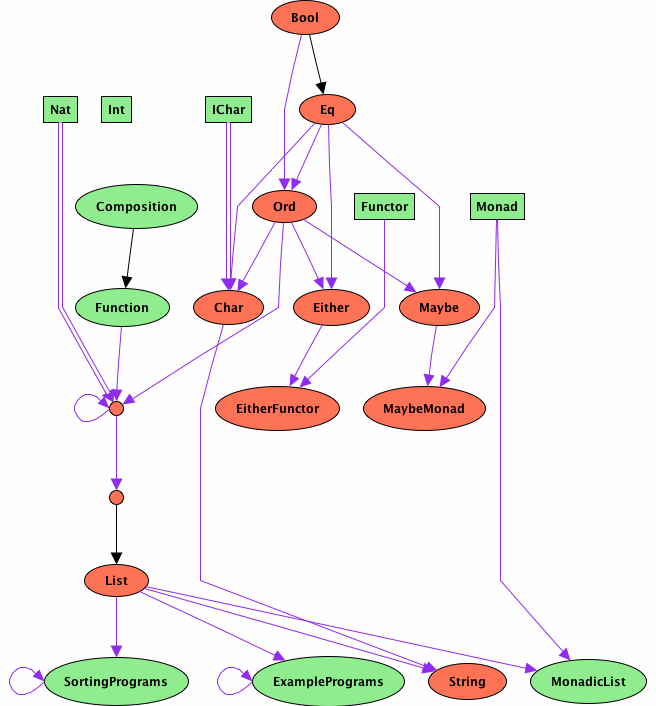
\includegraphics[scale=0.7]{ProofStart}
\caption{Initial state of the proof graph.}
\label{fig:Start}
\end{figure}

As can be seen, all the red (dark gray) nodes indicate specifications that have one or more theorems. The green (light gray) ones don't have theorems or, either, their proofs are already done. The rectangular nodes indicate imported specifications and the elliptical ones indicate specifications taken from our file. Some nodes, such as \verb.ExamplePrograms. and \verb.SortingPrograms., do have theorems but are marked green because the theorems are inserted in sub-specifications.

We started our proofs by using the automatic proof mode of \textit{Hets} (menu: Edit -> Proofs -> Automatic). This method analyzed the theories and directives (\verb.%mono., \verb.%implies, etc.) and then revealed the nodes from sub-specifications that created theorems, for example, by the \verb.%implied. directive.

The next step was to prove each red node. To do so, we did a right click on a node and chose the option \textit{Prove} from the \textit{node menu}. This opened the Emacs text editor. After \textit{Isabelle} had parsed the full theory file (and proved it or not, according to \textit{Isabelle} rules), we closed the Emacs window and thus the proof status for that theory was reported back to \textit{Hets} by \textit{Isabelle}. If the node was proved, its color changed to green; otherwise, it kept the red color. If sub-nodes were proved, they were omitted again by \textit{Hets}. At this point, we could not yet prove all the theorems we had created. Most of the unproved nodes had yet one or two theorems to be proved. The actual status of our proofs can be seen in \citeFig{fig:Status}.

\begin{figure}[htp]
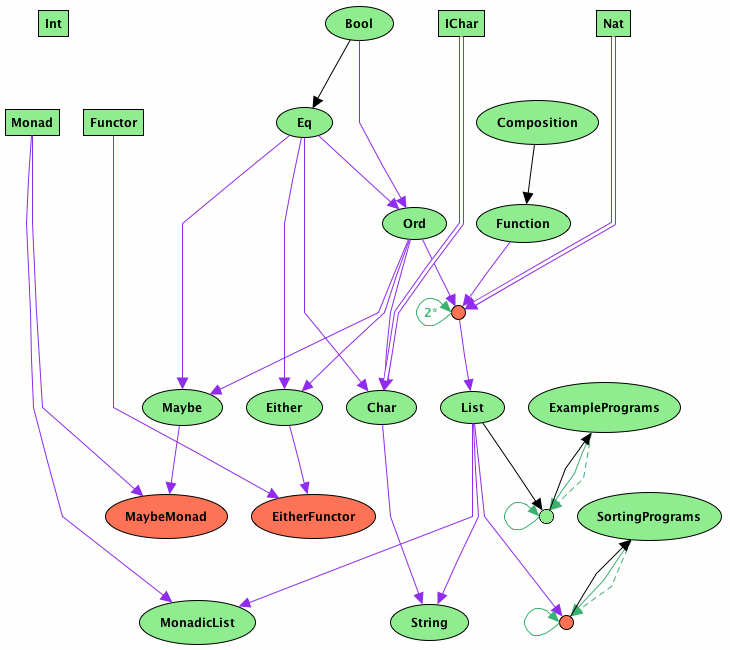
\includegraphics[scale=0.6]{ProofEnd}
\caption{Actual state of the proof graph.}
\label{fig:Status}
\end{figure}

\clearpage

\subsection{Verifying specifications with Isabelle}
As part of specifying our library, the task of proving its theorems were a major undertaking. Although some theorems remained unproved, we verified almost all of them. Next, we indicate how we constructed our proofs using excerpts from interesting proofs. Our full proof scripts can be found in \citeAppendix.

The four theorems from \citeSpec{spec:Bool}, were translated by \textit{Hets} to \textit{Isabelle} theorems like the one shown by \citeProof{proof:Bool}.

\begin{proof}
\begin{verbatim}
theorem NotFalse1 : "ALL x. Not' x = True' = (x = False')"
apply auto
apply (case_tac x)
apply auto
done
\end{verbatim}
\caption{Proof for theorem NotFalse1 from Bool specification}
\label{proof:Bool}
\end{proof}

All the proofs for the theorems of the \verb.Bool. specification followed this pattern:
\begin{itemize}
\item \textit{apply (auto)}:

This command tries to simplify the actual goal automatically, and as deep as it can. In this case, the command could only eliminate the universal quantifier, getting the result:
\begin{verbatim}
goal (1 subgoal):
 1. !!x. Not' x = True' ==> x = False'
\end{verbatim}

\item \textit{apply (case\_tac x)}:

case\_tac method executes a case distinction over all constructors of the data type of variable \verb.x.. In this case, because the type of \verb.x. is \verb.Bool., \verb.x. was instantiated to \verb.True. and \verb.False.:
\begin{verbatim}
goal (2 subgoals):
 1. !!x. [| Not' x = True'; x = False' |]
         ==> x = False'
 2. !!x. [| Not' x = True'; x = True' |]
         ==> x = False'
\end{verbatim}

\item \textit{apply (auto)}:

At this time, this command could finalize all the proof automatically. 
\begin{verbatim}
goal:
No subgoals!
\end{verbatim}
\end{itemize}

One example of a proof for an \verb.Eq. theorem is shown in the \citeProof{proof:Eq}. In this proof, we used a new command: \verb.simp add:.. This command expects a list of axioms and previously proved theorems as parameters to be used in an automatic tentative of proving the actual goal. This command uses other axioms from the theory, together with the theorems passed as parameters, when trying to simplify the goal. If the goal cannot be reduced, the command produces an error; otherwise, a new goal is received.

\begin{proof}
\begin{verbatim}
theorem DiffTDef :
"ALL x. ALL y. x /= y = True' = (Not' (x ==' y) = True')"
apply(auto)
apply(simp add: DiffDef)
apply(case_tac "x ==' y")
apply(auto)
apply(simp add: DiffDef)
done
\end{verbatim}
\caption{Equality proof}
\label{proof:Eq}
\end{proof}

Almost all Ord theorem proofs used the same commands and tactics from the previous proofs. One interesting proof was the one for the axiom \axiom{LeTAsymmetry}, presented in the \citeProof{proof:Ord}. Sometimes, \textit{Isabelle} expected us to rewrite axioms to match goals because it cannot change the axioms to all their equivalent forms. We applied the command \verb.rule ccontr. to start a proof by contradiction. After some simplification, \textit{Isabelle} was not able to use the axiom \axiom{LeIrreflexivity} to simplify the goal:

\begin{verbatim}
goal (1 subgoal):
 1. !!x y. [| x <' y = True'; y <' x = True' |] ==> False
\end{verbatim}

We needed to define an auxiliary lemma, \verb.LeIrreflContra., which \textit{Isabelle} automatically proved. This theorem is interpreted internally by \textit{Isabelle} as:

\begin{verbatim}
?x <' ?x = True' ==> False
\end{verbatim}

Hence, we could tell \textit{Isabelle} to use this lemma, thus forcing it to attribute the variable \verb.x. to each \verb.?x. variable in the lemma using the command \verb.rule_tac x="x". \verb.in LeIrreflContra.. The same tactic was used to force the use of the axiom \axiom{LeTTransitive}. The command \verb.by auto. was used to finalize the proof.

\begin{proof}
\begin{verbatim}
lemma LeIrreflContra : " x <' x = True' ==> False"
by auto

theorem LeTAsymmetry :
"ALL x. ALL y. x <' y = True' --> y <' x = False'"
apply(auto)
apply(rule ccontr)
apply(simp add: notNot2 NotTrue1)
apply(rule_tac x="x" in LeIrreflContra)
apply(rule_tac y="y" in LeTTransitive)
by auto
\end{verbatim}
\caption{Proof for the axiom LeTAsymmetry from specification Ord.}
\label{proof:Ord}
\end{proof}

We started most of our proofs by applying the command \verb.apply(auto)., as we wanted \textit{Isabelle} to act automatically as much as possible. Sometimes this command could do some reductions. Sometimes it could only remove \textit{HOL} universal quantifiers. Sometimes it got into a loop.

An example of a loop occurred when proving theorems from the \verb.Maybe. and \verb.Either. specifications. To avoid the loop, we applied the universal quantifier rule directly, using the command \verb.apply(rule allI).. The command \verb.rule. applies the specified theorem directly. When there were more than one quantified variable, we could use the \verb.+. sign after the rule, in order  to tell \textit{Isabelle} to apply the command as many times as it could.

After we removed the quantifiers, we could use the command \verb.simp only:. to do some simplification. Differently from \verb.simp add:., the command \verb.simp only:. rewrites only the rules passed as parameters when simplifying the actual goal. Most of the time they could be used interchangeably. Sometimes, however, \verb.simp add:. got into a loop and \verb.simp only:. had to be used with other proof commands. Two theorems from the\verb.Maybe. specification exemplify the use of the previous commands, as shown in the \citeProof{proof:Maybe}.

\begin{proof}\capstart
\begin{verbatim}
theorem IMO05 : "ALL x. Just(x) <' Nothing = False'"
apply(rule allI)
apply(case_tac "Just(x) <' Nothing")
apply(auto)
done

theorem IMO08 :
"ALL x. compare Nothing (Just(x)) ==' GT = Nothing >' Just(x)"
apply(rule allI)+
apply(simp add: GeDef)
done
\end{verbatim}
\caption{Proof for theorems IMO05 and IMO08 from specification Maybe.}
\label{proof:Maybe}
\end{proof}

The \verb.List. specification still had unproved theorems (\verb.FoldlDecomp. and \verb.ZipSpec.) inside one of its sub-nodes. The other nodes could have all its theorems proved. Almost all theorems in this specification needed induction to be proved. \textit{Isabelle} executes induction over a specified variable using the command \verb.induct_tac.. it expects as parameter an expression or a variable over which to execute the induction. In the \citeProof{proof:List}, we can see one example of proof by induction for a \verb.List. theorem.

\begin{proof}\capstart
\begin{verbatim}
theorem FilterProm :
"ALL f.
 ALL p.
 ALL xs.
 X_filter p (X_map f xs) = X_map f (X_filter (X__o__X (p, f)) xs)"
apply(auto)
apply(induct_tac xs)
apply(auto)
apply(case_tac "p(f a)")
apply(auto)
apply(simp add: MapCons)
apply(simp add: FilterConsT)
apply(simp add: MapCons)
apply(simp add: FilterConsT)
done
\end{verbatim}
\caption{Proof for theorem FilterProm from specification List.}
\label{proof:List}
\end{proof}

The specification \verb.Char. was another case where we had to use the \verb.rule. command to remove universal quantification by hand in order to avoid loops. Besides this problem, all theorems needed only one or two applications of the command \verb. simp add:. to be proved. An example can be seen in the \citeProof{proof:Char}.

\begin{proof}\capstart
\begin{verbatim}
theorem ICO07 : "ALL x. ALL y. ord'(x) >='' ord'(y) = x >='' y"
apply(rule allI)+
apply(simp only: GeqDef)
apply(simp add: GeDef)
done
\end{verbatim}
\caption{Proof for theorem ICO07 from specification Char.}
\label{proof:Char}
\end{proof}

The specification for \verb.String. also used few commands in order to have its theorems proved. Almost all proofs were done with combinations of the \verb.auto. and the \verb.simp add:. commands. the In \citeProof{proof:String}, we show the largest proof in the \verb.String. theory.

\begin{proof}\capstart
\begin{verbatim}
theorem StringT2 :
"ALL x.
 ALL xs.
 ALL y.
 ALL ys. xs /= ys = True' --> X_Cons x ys ==' X_Cons y xs = False'"
apply(auto)
apply(simp add: ILE02)
apply(case_tac "x ==' y")
apply(auto)
apply(simp add: EqualSymDef)
apply(simp add: DiffDef)
apply(simp add: NotFalse1)
done
\end{verbatim}
\caption{Proof for theorem StringT2 from specification String.}
\label{proof:String}
\end{proof}

Proofs of the \verb.ExamplePrograms. theorems were very long. They were done using basically three commands: \verb.simp only:., \verb.case_tac. and \verb.simp add:.. The latter was used as the last command to allow \textit{Isabelle} finish the proofs with fewer commands. Before the \verb.simp only:. applications, we tried the \verb.simp add:. command without success. We then used the \verb.simp only:. command directly when the theorem used previously as a parameter failed when using the \verb.simp add:. command. In the \citeProof{proof:ExamplePrograms}, we show the proof for an \verb.insertionSort. function application.

\begin{proof}\capstart
\begin{verbatim}
theorem Program03 :
"insertionSort(X_Cons True' (X_Cons False' Nil')) =
 X_Cons False' (X_Cons True' Nil')"
apply(simp only: InsertionSortConsCons)
apply(simp only: InsertionSortNil)
apply(simp only: InsertNil)
apply(case_tac "True' >'' False'")
apply(simp only: GeFLeTEqTRel)
apply(simp add: LeqTLeTEqTRel)
apply(simp only: InsertCons2)
apply(simp only: InsertNil)
done
\end{verbatim}
\caption{Proof for theorem Program03, an example of insertionSort function application from specification ExamplePrograms.}
\label{proof:ExamplePrograms}
\end{proof}

All the theorems from our last proof, \verb.SortingPrograms., still couldn't be proved. Although for all of them we could prove some goals, the last one, representing the general case, is yet unproved. To show our progress in the proofs, we present an example in the \citeProof{proof:SortingPrograms}, with some comments inserted. The command \verb.prefer. is used to choose which goal to prove in \textit{Isabelle} interactive mode, and the command \verb.oops. indicates that we could not prove the theorem, and that we gave up the proof.

\begin{proof}[tb]\capstart
\begin{verbatim}
theorem Theorem07 : "ALL xs. isOrdered(insertionSort(xs))"
apply(auto)
apply(case_tac xs)
(* Proof for xs=Nil *)
prefer 2
apply(simp only: InsertionSort)
apply(simp add: GenSortF)
(* Proof for general case *)
apply(simp only: InsertionSort)
apply(case_tac List)
apply(auto)
apply(case_tac "X_splitInsertionSort (X_Cons a (X_Cons aa Lista))")
(* Proof for xs= Cons a Nil *)
prefer 2
apply(simp add: GenSortF)
(* Proof for xs=Cons a as*)
apply(case_tac Lista)
apply(auto)
prefer 2
(* Proof for xs = Cons a (Cons b Nil)*)
oops
\end{verbatim}
\caption{Actual status of the proof for theorem Theorem07 of specification SortingPrograms.}
\label{proof:SortingPrograms}
\end{proof}

\section{Discussion and difficulties}\label{Discussion}
We faced some interesting difficulties that we will briefly discuss here. The first problem was dealing with the \textit{HasCASL} and \textit{CASL} languages. Although both languages can be used together, we intended to use the \textit{HasCASL} features, but separating both syntax were a little troublesome. The \textit{HasCASL} language doesn't yet have a definitive and complete manual as does the \textit{CASL} language. So, we started reading the \textit{CASL} manual and then the \textit{HasCASL} definitions. This created some difficulties when using the \textit{HasCASL} syntax because some of the constructions may be used interchangeably between both languages.

Another difficulty was when distinguishing between the logic relations of the \textit{HasCASL} language and our functions. This relates to the logical equivalence between some axioms. Although these axioms were equivalent, their uses as rewriting rules were different. Axioms could be defined by equality, as in
\begin{verbatim}
. (x > y) = (y < x)
\end{verbatim}

or by \textit{HasCASL} equivalence, as in
\begin{verbatim}
. (x > y) = True  <=> (y < x) = True
\end{verbatim}

The first case is a better choice when using axioms and theorems to refine rewrite rules into basic axioms. The second case must be used then defining basic axioms. Otherwise, \textit{Isabelle} will never be able to use these axioms. This relates to the fact that axioms defining relations should use the \verb.Bool. type to allow \textit{Isabelle} to conclude that rules are true or false and, then, proceed to prove goals.

We had some problems dealing with \textit{Isabelle} itself. We started using \textit{HOL} in place of \textit{Isar} and this seems to have complicated some proof scripts of larger proofs. We also had to get used to the way \textit{Isabelle} uses axioms as rewriting rules. If a predicate P implies a predicate Q (\verb.P ==> Q.), \textit{Isabelle} matches the predicate Q with the actual goal, constructing the proof in a bottom up manner that is not usual.

As \textit{HasCASL} is a work-in-progress project, the tool is not fully implemented and we got some errors because the tool could not translate some specifications to \textit{HOL}. Solutions to those errors were kindly proposed by the \textit{HasCASL} research team, thus minimizing our difficulties.

\section{Related Frameworks}\label{RelatedFrameworks}
There are other formal specification frameworks available. All of them include example libraries, to serve as a basis for new specifications, or predefined libraries, to be imported by larger specifications.

\textit{Larch}~\citep{LarchBook} and \textit{VSE-2}~\citep{VSE} are two examples of specification languages based on first-order logic. \textit{VDM}~\citep{VDM} and \textit{Z}~\citep{ZNotation} are model-oriented specification languages, i.e., their specifications model a single input-output behavior. \textit{HasCASL}, in contrast, contains loose specifications that can model a variety of similar behaviors in an abstract manner, allowing them to be refined later. \textit{CafeOBJ}~\citep{CafeOBJReport} and \textit{Maude}~\citep{MaudeLib} are specification languages that are directly executable; the price paid for this property is the reduced expressiveness of their logic in comparison with \textit{HasCASL}.

\textit{Extended ML}~\citep{SML} creates a higher order specification language on top of the programming language \textit{ML}. This approach resulted in a large language that is very difficult to manage. Similar approach was taken by the \textit{Programatica} framework~\citep{ProgramaticaOverview}, which provides a specification logic for the \textit{Haskell} language, called \textit{P-logic}. The similarities between \textit{HasCASL} and \textit{P-logic} includes the support for polymorphism and recursion based on an axiomatic treatment of complete partial orders. Because \textit{P-logic} is built directly on top of Haskell, it is less general than \textit{HasCASL}. This means that one \textit{HasCASL} specification can be loosely specified with generic higher order logic in mind and later refined to the logic of \textit{Haskell} programs. In opposite, \textit{P-logic} can only specify objects in the logic of \textit{Haskell} programs, including all its specialities, such as laziness. \textit{HasCASL} also includes support for class based overloading and constructor classes, needed for the specification of monads, and the Hoare logic for imperative (monad-based) programs.

Other higher order frameworks for software specification include \textit{Spectrum}~\citep{Spectrum} and \textit{RAISE}~\citep{RaiseSpecification}. The first is considered a precursor of \textit{HasCASL} and differs from it by using a three-valued logic and by limiting higher order mechanisms to continuous functions, as it doesn't have a proper higher-order specification language. The language of the \textit{RAISE} framework differs from \textit{HasCASL} because of the three-valued logic and the lack of support for polymorphism.

\section{Future Works}\label{FutureWorks}
As presented before, our library still has some incomplete proofs and some \textit{Haskell Prelude} functions still need to be specified. Presently, we are trying to finish the open proofs in order to get a fully verified subset of the \textit{Haskell Prelude} functions.

%TODO: encontrar a citação para a solução do isomorfismo já feito e dizer que ele precisa ser reescrito para ser usado com as ferramentas atuais.
An open question is how to deal with numbers. The alternative of recreating all the lemmas needed by \textit{Isabelle}, which are already written in \textit{HOL}, definitely is not a good approach. One solution could be to create an isomorphism between the builtin \textit{Isabelle} numeric types and the types specified in the \textit{CASL} library. If we call this isomorphism \verb.h., we could prove a goal like \verb.t1 = t2. by injecting the isomorphism using the rule \verb.h x = h y ==> x = y.. This axiom would give us a new goal, \verb.h t1 = h t2., that would be written in terms of builtin \textit{Isabelle} types and, thus, could be proved with the \textit{Isabelle} axioms and builtin auxiliary lemmas. This isomorphism could be extended to the specification \verb.List., as most \textit{Haskell} data types and functions rely on lists.

After solving the problem with numeric specifications, we could specify the \textit{Haskell Prelude} functions that involve numbers. Many functions that should have been specified on the specification \verb.List., for example, are absent because importing the numeric specifications wouldn't allow their proofs to be constructed.

The next natural stage would be to use laziness in our library. This would require a rewrite of almost all the specifications. An alternative would be to study transformations that could help us to reuse the proofs we have already written.

Another point of interest would be to refine our library in order to use the \textit{HasCASL} language subset. This subset contains structures like infinite data types and allows specifications to be converted to \textit{Haskell} programs. This last step could also be used to verify existing \textit{Haskell Prelude} implementations or to serve as a guide for new ones.

\section{Conclusions}\label{Conclusions}
In this report, we described some first steps towards specifying a library for the \textit{HasCASL} language. The specification was based on the \textit{Prelude} library, from the \textit{Haskell} language. We focused on describing our technical choices and on discussing implementation details.

We specified a major part of the \textit{Prelude} library, including almost all the data types and various functions. We decided to use strict types because a future refinement can modify the library to include laziness. We proved almost all the proposed theorems from our specifications using the \textit{Isabelle} tool.

Although we didn't use the \textit{HasCASL}'s subset that can be translated to \textit{Haskell} programs, our specification can be used to specify small programs involving basic data types and structures. To exemplify, we presented two specifications involving sorting algorithms over lists.

An open issue is how to deal with numbers. Although numeric specifications can be imported from the \textit{CASL} library to write specifications, this libraries cannot be used to write proofs in \textit{Isabelle} because they lack auxiliary theorems that the prover needs to use as rewrite rules. The solution we found to circumvent to this problem involved the rewriting of large pieces of code in order for it to be used in the present stage of the tools.

Future steps could involve the the study of rules to refine the specifications in order to include laziness and infinite data types. Another point of interest would be to use the subset of the \textit{HasCASL} language that can generate \textit{Haskell} programs.

\bibliography{TechReportMSc,cofi}

\clearpage

\appendix
\appendixpage
\section{Isabelle Proof Scripts}
\label{appendix:proofs}
We transcribed here the proof contents of each theory file generated by Hets. For a question of readability, we didn't transcribed the automatic generated sections of each theory, as they can be regenerated with our previous listed specifications.

%Index for Proof Scripts
\newcounter{appindex}

\begin{multicols}{2}
\addtocounter{appindex}{1}
\large{\textbf{Isabelle Proof Script \thesection{}.\theappindex{}} Prelude\_Bool.thy}

\label{pscript:Bool}
\tiny
\begin{verbatim}
theorem NotFalse1 : "ALL x. Not' x = True' = (x = False')"
apply auto
apply(case_tac x)
apply auto
done
ML "Header.record \"NotFalse1\""

theorem NotTrue1 : "ALL x. Not' x = False' = (x = True')"
apply auto
apply(case_tac x)
apply auto
done
ML "Header.record \"NotTrue1\""

theorem notNot1 : "ALL x. (~ x = True') = (Not' x = True')"
apply(auto)
apply(case_tac x)
apply(auto)
done
ML "Header.record \"notNot1\""

theorem notNot2 : "ALL x. (~ x = False') = (Not' x = False')"
apply(auto)
apply(case_tac x)
apply(auto)
done
ML "Header.record \"notNot2\""

end
\end{verbatim}
\end{multicols}

\begin{multicols}{2}
\addtocounter{appindex}{1}
\large{\textbf{Isabelle Proof Script \thesection{}.\theappindex{}} Prelude\_Eq.thy}
\label{pscript:Eq}
\tiny
\begin{verbatim}
theorem DiffSymDef : "ALL x. ALL y. x /= y = y /= x"
apply(auto)
apply(simp add: DiffDef)
apply(simp add: EqualSymDef)
done
ML "Header.record \"DiffSymDef\""

theorem DiffTDef :
"ALL x. ALL y. x /= y = True' = (Not' (x ==' y) = True')"
apply(auto)
apply(simp add: DiffDef)
apply(case_tac "x ==' y")
apply(auto)
apply(simp add: DiffDef)
done
ML "Header.record \"DiffTDef\""

theorem DiffFDef :
"ALL x. ALL y. x /= y = False' = (x ==' y = True')"
apply(auto)
apply(simp add: DiffDef)
apply(case_tac "x ==' y")
apply(auto)
apply(simp add: DiffDef)
done
ML "Header.record \"DiffFDef\""

theorem TE1 : "ALL x. ALL y. x ==' y = False' --> ~ x = y"
by auto
ML "Header.record \"TE1\""

theorem TE2 :
"ALL x. ALL y. Not' (x ==' y) = True' = (x ==' y = False')"
apply auto
apply(case_tac "x ==' y")
apply auto
done
ML "Header.record \"TE2\""

theorem TE3 :
"ALL x. ALL y. Not' (x ==' y) = False' = (x ==' y = True')"
apply(auto)
apply(case_tac "x ==' y")
apply auto
done
ML "Header.record \"TE3\""

theorem TE4 :
"ALL x. ALL y. (~ x ==' y = True') = (x ==' y = False')"
apply auto
apply(case_tac "x ==' y")
apply auto
done

ML "Header.record \"TE4\""

theorem IBE1 : "True' ==' True' = True'"
by auto
ML "Header.record \"IBE1\""

theorem IBE2 : "False' ==' False' = True'"
by auto
ML "Header.record \"IBE2\""

theorem IBE4 : "True' ==' False' = False'"
apply(simp add: EqualSymDef)
done
ML "Header.record \"IBE4\""

theorem IBE5 : "True' /= False' = True'"
apply(simp add: DiffDef)
apply(simp add: IBE4)
done
ML "Header.record \"IBE5\""

theorem IBE6 : "False' /= True' = True'"
apply(simp add: DiffDef)
done
ML "Header.record \"IBE6\""

theorem IBE7 : "Not' (True' ==' False') = True'"
apply(simp add: IBE4)
done
ML "Header.record \"IBE7\""

theorem IBE8 : "Not' Not' (True' ==' False') = False'"
apply(simp add: IBE4)
done
ML "Header.record \"IBE8\""

theorem IUE1 : "() ==' () = True'"
by auto
ML "Header.record \"IUE1\""

theorem IUE2 : "() /= () = False'"
apply(simp add: DiffDef)
done
ML "Header.record \"IUE2\""

end
\end{verbatim}
\end{multicols}

\begin{multicols}{2}
\addtocounter{appindex}{1}
\large{\textbf{Isabelle Proof Script \thesection{}.\theappindex{}} Prelude\_Ord.thy}
\label{pscript:Ord}
\tiny
\begin{verbatim}
theorem IOE01 : "LT ==' LT = True'"
by auto
ML "Header.record \"IOE01\""

theorem IOE02 : "EQ ==' EQ = True'"
by auto
ML "Header.record \"IOE02\""

theorem IOE03 : "GT ==' GT = True'"
by auto
ML "Header.record \"IOE03\""

theorem IOE07 : "LT /= EQ = True'"
apply(simp add: DiffDef)
done
ML "Header.record \"IOE07\""

theorem IOE08 : "LT /= GT = True'"
apply(simp add: DiffDef)
done
ML "Header.record \"IOE08\""

theorem IOE09 : "EQ /= GT = True'"
apply(simp add: DiffDef)
done
ML "Header.record \"IOE09\""

lemma LeIrreflContra : " x <' x = True' ==> False"
by auto

theorem LeTAsymmetry :
"ALL x. ALL y. x <' y = True' --> y <' x = False'"
apply(auto)
apply(rule ccontr)
apply(simp add: notNot2 NotTrue1)
thm LeIrreflContra
apply(rule_tac x="x" in LeIrreflContra)
apply(rule_tac y = "y" in LeTTransitive)
by auto
ML "Header.record \"LeTAsymmetry\""

theorem GeIrreflexivity :
"ALL x. ALL y. x ==' y = True' --> x >' y = False'"
apply(auto)
apply(simp add: GeDef)
apply(simp add: EqualSymDef LeIrreflexivity)
done
ML "Header.record \"GeIrreflexivity\""

theorem GeTAsymmetry :
"ALL x. ALL y. x >' y = True' --> y >' x = False'"
apply(auto)
apply(simp add: GeDef)
apply(simp add: LeTAsymmetry)
done
ML "Header.record \"GeTAsymmetry\""

theorem GeTTransitive :
"ALL x.
 ALL y. ALL z. (x >' y) && (y >' z) = True' --> x >' z = True'"
apply(auto)
apply(simp add: GeDef)
apply(rule_tac x="z" and y="y" and z="x" in  LeTTransitive)
apply(auto)
apply(case_tac  "z <' y")
apply(auto)
apply(case_tac  "y <' x")
apply(auto)
apply(case_tac  "y <' x")
apply(auto)
done
ML "Header.record \"GeTTransitive\""

theorem GeTTotal :
"ALL x. ALL y. ((x >' y) || (y >' x)) || (x ==' y) = True'"
apply(auto)
apply(simp add: OrDef)
apply(case_tac "x >' y")
apply(auto)
apply(case_tac "y >' x")
apply(auto)
apply(case_tac "x ==' y")
apply(auto)
apply(simp add: GeDef)
apply(simp add: LeFGeTEqTRel)
apply(auto)
apply(simp add: GeDef)
apply(simp add: LeTAsymmetry)
apply(simp add: EqualSymDef)
done
ML "Header.record \"GeTTotal\""

theorem LeqReflexivity : "ALL x. x <=' x = True'"
apply(auto)
apply(simp add: LeqDef)
apply(simp add: OrDef)
done
ML "Header.record \"LeqReflexivity\""

lemma EqualL1 [rule_format]:
"ALL x z.
 ((x ==' z) = True') & ((x ==' z) = False') \<longrightarrow> False"
by auto

lemma EqualL2 [rule_format]:
"ALL x. ALL y. ALL z.
((x ==' y) = True') & ((y ==' z) = True') \<longrightarrow>
((x ==' z) = False')\<longrightarrow> False"
apply(simp add: EqualL1)
apply(simp add: notNot2 NotTrue1)
apply(auto)
apply(rule EqualTransT)
apply(auto)
done

lemma Le1E [rule_format]:
"ALL x y z.
(y ==' x) = True' & (x <' z) = True' \<longrightarrow> (y <' z) = True'"
apply (auto)
apply(rule EqTOrdTSubstE)
apply(auto)
done

lemma Le2 [rule_format]:
"ALL x y.
(x <' y) = True' \<longrightarrow> (x <' y) = False'
\<longrightarrow> False"
by auto

lemma Le3E [rule_format]:
"ALL x y z.
(y ==' x) = True' & (x <' z) = True' \<longrightarrow> (y <' z) = False'
\<longrightarrow> False"
apply (auto)
apply(rule Le2)
apply(rule EqTOrdTSubstE)
apply(auto)
done

lemma Le3D [rule_format]:
"ALL x y z.
(y ==' x) = True' & (z <' x) = True' \<longrightarrow> (z <' y) = False'
\<longrightarrow> False"
apply (auto)
apply(rule Le2)
apply(rule EqTOrdTSubstD)
apply(auto)
done

lemma Le4E [rule_format]:
"ALL x y z.
(y ==' x) = True' & (x <' z) = False' \<longrightarrow> (y <' z) = False'"
apply (auto)
apply(rule EqTOrdFSubstE)
apply(auto)
done

lemma Le4D [rule_format]:
"ALL x y z.
(y ==' x) = True' & (z <' x) = False' \<longrightarrow> (z <' y) = False'"
apply (auto)
apply(rule EqTOrdFSubstD)
apply(auto)
done

lemma Le5 [rule_format]:
"ALL x y.
(x <' y) = False' \<longrightarrow> (x <' y) = True'
\<longrightarrow> False"
by auto

lemma Le6E [rule_format]:
"ALL x y z.
(y ==' x) = True' & (x <' z) = False' \<longrightarrow> (y <' z) = True'
\<longrightarrow> False"
apply (auto)
apply(rule Le5)
apply(rule EqTOrdFSubstE)
apply(auto)
done

lemma Le7 [rule_format]:
"ALL x y.
x <' y = True' & x <' y = False' \<longrightarrow> False"
by auto

theorem LeqTTransitive :
"ALL x.
 ALL y. ALL z. (x <=' y) && (y <=' z) = True' --> x <=' z = True'"
apply(auto)
apply(simp add: LeqDef)
apply(simp add: OrDef)
apply(case_tac "x <' y")
apply(auto)
apply(case_tac "x ==' y")
apply(auto)
apply(case_tac "y <' z")
apply(auto)
apply(case_tac "y ==' z")
apply(auto)
apply(case_tac "x <' z")
apply(auto)
apply(case_tac "x ==' z")
apply(auto)
(*Here we needed the first aux lemma*)
apply(rule EqualL2)
apply(auto)
apply(simp add: NotFalse1 NotTrue1)
apply(case_tac "Not' (x <' z)")
apply(simp add: AndFalse)
apply(simp add: NotFalse1 NotTrue1)
apply(rule ccontr)
apply(simp add: notNot1 NotFalse1)
apply(erule Le2)
apply(rule Le4E)
apply(auto)
apply(simp add: EqualSymDef)
(*End of the proof of the first thm that needed an aux lemma*)
apply(case_tac "y <' z")
apply(auto)
apply(case_tac "y ==' z")
apply(auto)
apply(case_tac "x <' z")
apply(auto)
apply(case_tac "x ==' z")
apply(auto)
(*From now on I guess the proof must be verified. It seems that I 
inserted some loops in the proof. *)
apply(simp add: LeTGeFEqFRel)
apply(auto)
apply(simp add: LeFGeTEqTRel)
apply(simp add: EqTSOrdRel)
apply(simp add: EqFSOrdRel)
apply(auto)
apply(simp add: GeDef)
apply(simp add: LeTGeFEqFRel LeFGeTEqTRel)
apply(auto)
apply(simp add: GeDef)
apply(simp add: LeTAsymmetry LeIrreflexivity LeTTotal)
apply(simp add: GeDef)+
(*
apply(simp add: GeDef)
apply(simp add: GeDef)
*)
apply(simp add: EqualSymDef LeTGeFEqFRel LeFGeTEqTRel )
apply(simp add: GeDef)
(*The real proof seems to be in the next 3 lines.*)
apply(rule Le3E)
apply(auto)
apply(simp add: EqualSymDef)+
(*
apply(simp add: EqualSymDef)
apply(simp add: EqualSymDef)
apply(simp add: EqualSymDef)
*)
(*Verify until here.*)
(*The proof for the last goal.*)
apply(case_tac "x <' y")
apply(auto)
apply(case_tac "x <' z")
apply(auto)
apply(case_tac "x ==' z")
apply(auto)
apply(drule Le5)
apply(rule LeTTransitive)
apply(auto)
done
ML "Header.record \"LeqTTransitive\""

theorem LeqTTotal :
"ALL x. ALL y. (x <=' y) && (y <=' x) = x ==' y"
apply(auto)
apply(simp add: LeqDef)
apply(simp add: OrDef)
apply(case_tac "x <' y")
apply(auto)
apply(case_tac "x ==' y")
apply(auto)
apply(case_tac "x ==' y")
apply(auto)
apply(case_tac "y <' x")
apply(auto)
apply(case_tac "y ==' x")
apply(auto)
apply(case_tac "y ==' x")
apply(auto)
apply(case_tac "y <' x")
apply(auto)
apply(case_tac "y ==' x")
apply(auto)
apply(simp add: EqualSymDef)
apply(simp add: EqualSymDef)
apply(case_tac "x ==' y")
apply(auto)
apply(case_tac "y <' x")
apply(auto)
apply(case_tac "y ==' x")
apply(auto)
apply(simp add: LeTAsymmetry)
done
ML "Header.record \"LeqTTotal\""

theorem GeqReflexivity : "ALL x. x >=' x = True'"
apply(auto)
apply(simp add: GeqDef)
apply(simp add: GeDef)
apply(simp add: OrDef)
done
ML "Header.record \"GeqReflexivity\""

theorem GeqTTransitive :
"ALL x.
 ALL y. ALL z. (x >=' y) && (y >=' z) = True' --> x >=' z = True'"
apply(auto)
apply(simp add: GeqDef)
apply(simp add: OrDef GeDef)
apply(case_tac "y <' x")
apply(auto)
apply(case_tac "x ==' y")
apply(auto)
apply(case_tac "z <' y")
apply(auto)
apply(case_tac "y ==' z")
apply(auto)
apply(case_tac "z <' x")
apply(auto)
apply(case_tac "x ==' z")
apply(auto)
(*Here we needed the first aux lemma*)
apply(rule EqualL2)
apply(auto)
apply(simp add: NotFalse1 NotTrue1)
apply(case_tac "Not' (z <' x)")
apply(simp add: AndFalse)
apply(simp add: NotFalse1 NotTrue1)
apply(rule ccontr)
apply(simp add: notNot1 NotFalse1)
apply(erule Le2)
apply(rule EqTOrdFSubstD)
apply(auto)
apply(simp add: EqualSymDef)
(*End of the proof of the first thm that needed an aux lemma*)
apply(case_tac "z <' y")
apply(auto)
apply(case_tac "y ==' z")
apply(auto)
apply(case_tac "z <' x")
apply(auto)
apply(case_tac "x ==' z")
apply(auto)
(*From now on I guess the proof must be verified. It seems that I
inserted some loops in the proof. *)
apply(simp add: LeTGeFEqFRel)
apply(auto)
apply(simp add: LeFGeTEqTRel)
apply(simp add: EqTSOrdRel)
apply(simp add: EqFSOrdRel)
apply(auto)
apply(simp add: GeDef)+
apply(simp add: LeFGeTEqTRel LeTGeFEqFRel)
apply(auto)
apply(simp add: GeDef)
apply(simp add: LeTAsymmetry LeIrreflexivity LeTTotal)
apply(simp add: GeDef)+
apply(simp add: EqualSymDef LeTGeFEqFRel LeFGeTEqTRel )
apply(simp add: GeDef)
(*The real proof seems to be in the next 3 lines.*)
apply(rule Le3D)
apply(auto)
apply(simp add: EqualSymDef)+
(*Verify until here.*)
apply(simp add: GeDef)+
apply(simp add: LeTAsymmetry)
apply(simp add: GeDef)+
(*The proof for the last goal.*)
apply(case_tac "z <' x")
apply(auto)
apply(case_tac "x ==' z")
apply(auto)
apply(drule Le5)
apply(rule LeTTransitive)
apply(auto)
done
ML "Header.record \"GeqTTransitive\""

theorem GeqTTotal :
"ALL x. ALL y. (x >=' y) && (y >=' x) = x ==' y"
apply(auto)
apply(simp add: GeqDef)
apply(simp add: OrDef)
apply(case_tac "x >' y")
apply(auto)
apply(case_tac "x ==' y")
apply(auto)
apply(case_tac "y >' x")
apply(auto)
apply(case_tac "y ==' x")
apply(auto)
apply(case_tac "y ==' x")
apply(auto)
apply(case_tac "y >' x")
apply(auto)
apply(case_tac "y ==' x")
apply(auto)
apply(simp add: EqualSymDef)
apply(simp add: EqualSymDef)
apply(case_tac "x ==' y")
apply(auto)
apply(case_tac "y >' x")
apply(auto)
apply(case_tac "y ==' x")
apply(simp add: GeDef)
apply(simp add: LeTAsymmetry)
apply(simp add: EqualSymDef)
apply(case_tac "y >' x")
apply(auto)
done
ML "Header.record \"GeqTTotal\""

theorem LeTGeTRel :
"ALL x. ALL y. x <' y = True' = (y >' x = True')"
apply(auto)
apply(simp add: GeDef)
apply(simp add: GeDef)
done
ML "Header.record \"LeTGeTRel\""

theorem LeFGeFRel :
"ALL x. ALL y. x <' y = False' = (y >' x = False')"
apply(auto)
apply(simp add: GeDef)
apply(simp add: GeDef)
done
ML "Header.record \"LeFGeFRel\""

theorem LeqTGetTRel :
"ALL x. ALL y. x <=' y = True' = (y >=' x = True')"
apply(auto)
apply(simp add: GeqDef LeqDef)
apply(simp add: OrDef)
apply(case_tac "y >' x")
apply(auto)
apply(case_tac "y ==' x")
apply(auto)
apply(case_tac "x <' y")
apply(auto)
apply(case_tac "x ==' y")
apply(auto)
apply(simp add: EqualSymDef)
apply(simp add: GeDef)
apply(simp add: GeqDef LeqDef)
apply(simp add: OrDef)
apply(case_tac "y >' x")
apply(auto)
apply(case_tac "y ==' x")
apply(auto)
apply(case_tac "x <' y")
apply(auto)
apply(case_tac "x ==' y")
apply(auto)
apply(simp add: EqualSymDef)
apply(case_tac "x <' y")
apply(auto)
apply(case_tac "x ==' y")
apply(auto)
apply(simp add: GeDef)
done
ML "Header.record \"LeqTGetTRel\""

theorem LeqFGetFRel :
"ALL x. ALL y. x <=' y = False' = (y >=' x = False')"
apply(auto)
apply(simp add: GeqDef LeqDef)
apply(simp add: OrDef)
apply(case_tac "x <' y")
apply(auto)
apply(case_tac "x ==' y")
apply(auto)
apply(case_tac "y >' x")
apply(auto)
apply(case_tac "y ==' x")
apply(auto)
apply(simp add: EqualSymDef)
apply(simp add: GeDef)
apply(simp add: GeqDef LeqDef)
apply(simp add: OrDef)
apply(case_tac "y >' x")
apply(auto)
apply(case_tac "y ==' x")
apply(auto)
apply(case_tac "x <' y")
apply(auto)
apply(case_tac "x ==' y")
apply(auto)
apply(simp add: EqualSymDef)
apply(simp add: GeDef)
done
ML "Header.record \"LeqFGetFRel\""

theorem GeTLeTRel :
"ALL x. ALL y. x >' y = True' = (y <' x = True')"
apply(auto)
apply(simp add: GeDef)
apply(simp add: GeDef)
done
ML "Header.record \"GeTLeTRel\""

theorem GeFLeFRel :
"ALL x. ALL y. x >' y = False' = (y <' x = False')"
apply(auto)
apply(simp add: GeDef)
apply(simp add: GeDef)
done
ML "Header.record \"GeFLeFRel\""

theorem GeqTLeqTRel :
"ALL x. ALL y. x >=' y = True' = (y <=' x = True')"
apply(auto)
apply(simp add: GeqDef LeqDef)
apply(simp add: OrDef)
apply(case_tac "x >' y")
apply(auto)
apply(case_tac "x ==' y")
apply(auto)
apply(case_tac "y <' x")
apply(auto)
apply(case_tac "y ==' x")
apply(auto)
apply(simp add: EqualSymDef)
apply(case_tac "y <' x")
apply(auto)
apply(case_tac "y ==' x")
apply(auto)
apply(simp add: GeDef)
apply(simp add: GeqDef LeqDef)
apply(simp add: OrDef)
apply(case_tac "y <' x")
apply(auto)
apply(case_tac "y ==' x")
apply(auto)
apply(case_tac "x >' y")
apply(auto)
apply(case_tac "x ==' y")
apply(auto)
apply(simp add: EqualSymDef)
apply(case_tac "x >' y")
apply(auto)
apply(case_tac "x ==' y")
apply(auto)
apply(simp add: GeDef)
done
ML "Header.record \"GeqTLeqTRel\""

theorem GeqFLeqFRel :
"ALL x. ALL y. x >=' y = False' = (y <=' x = False')"
apply(auto)
apply(simp add: GeqDef LeqDef)
apply(simp add: OrDef)
apply(case_tac "x >' y")
apply(auto)
apply(case_tac "x ==' y")
apply(auto)
apply(case_tac "y <' x")
apply(auto)
apply(case_tac "y ==' x")
apply(auto)
apply(simp add: EqualSymDef)
apply(simp add: GeDef)
apply(simp add: GeqDef LeqDef)
apply(simp add: OrDef)
apply(case_tac "y <' x")
apply(auto)
apply(case_tac "y ==' x")
apply(auto)
apply(case_tac "x >' y")
apply(auto)
apply(case_tac "x ==' y")
apply(auto)
apply(simp add: EqualSymDef)
apply(simp add: GeDef)
done
ML "Header.record \"GeqFLeqFRel\""

theorem LeqTGeFRel :
"ALL x. ALL y. x <=' y = True' = (x >' y = False')"
apply(auto)
apply(simp add: GeDef LeqDef OrDef)
apply(case_tac "x <' y")
apply(auto)
apply(case_tac "x ==' y")
apply(auto)
apply(simp add: EqualSymDef LeIrreflexivity)
apply(simp add: LeTAsymmetry)
apply(simp add: LeqDef OrDef)
apply(case_tac "x <' y")
apply(auto)
apply(case_tac "x ==' y")
apply(auto)
apply(simp add: EqFSOrdRel)
done
ML "Header.record \"LeqTGeFRel\""

theorem LeqFGeTRel :
"ALL x. ALL y. x <=' y = False' = (x >' y = True')"
apply(auto)
apply(simp add: GeDef LeqDef OrDef)
apply(case_tac "x <' y")
apply(auto)
apply(case_tac "x ==' y")
apply(auto)
apply(simp add: EqFSOrdRel)
apply(simp add: GeDef)
apply(simp add: LeqDef OrDef)
apply(case_tac "x <' y")
apply(auto)
apply(case_tac "x ==' y")
apply(auto)
apply(simp add: EqTSOrdRel)
apply(simp add: GeDef LeTAsymmetry)
done
ML "Header.record \"LeqFGeTRel\""

theorem GeTLeFEqFRel :
"ALL x.
 ALL y. x >' y = True' = (x <' y = False' & x ==' y = False')"
apply(auto)
apply(simp add: GeDef LeTAsymmetry)
apply(simp add: GeDef)
apply(simp add: EqFSOrdRel)
apply(auto)
apply(simp add: GeDef)
apply(simp add: EqFSOrdRel)
done
ML "Header.record \"GeTLeFEqFRel\""

theorem GeFLeTEqTRel :
"ALL x.
 ALL y. x >' y = False' = (x <' y = True' | x ==' y = True')"
apply(auto)
apply(simp add: LeTGeFEqFRel)
apply(simp add: notNot1)
apply(case_tac "x ==' y")
apply(auto)
apply(simp add: GeDef)
apply(simp add: LeTAsymmetry)
apply(simp add: GeDef)
apply(simp add: EqualSymDef LeIrreflexivity)
done
ML "Header.record \"GeFLeTEqTRel\""

theorem GeqTLeFRel :
"ALL x. ALL y. x >=' y = True' = (x <' y = False')"
apply(auto)
apply(simp add: GeqDef OrDef)
apply(case_tac "x >' y")
apply(auto)
apply(case_tac "x ==' y")
apply(auto)
apply(simp add: GeDef)
apply(simp add: LeTAsymmetry)
apply(simp add: GeqDef OrDef)
apply(case_tac "x >' y")
apply(auto)
apply(case_tac "x ==' y")
apply(auto)
apply(simp add: GeDef)
apply(simp add: EqFSOrdRel)
apply(simp add: GeDef)
done
ML "Header.record \"GeqTLeFRel\""

theorem GeqFLeTRel :
"ALL x. ALL y. x >=' y = False' = (x <' y = True')"
apply(auto)
apply(simp add: GeqDef OrDef)
apply(case_tac "x >' y")
apply(auto)
apply(case_tac "x ==' y")
apply(auto)
apply(simp add: GeDef)
apply(simp add: EqFSOrdRel)
apply(simp add: GeDef)
apply(simp add: GeqDef OrDef)
apply(case_tac "x >' y")
apply(auto)
apply(case_tac "x ==' y")
apply(auto)
apply(simp add: GeDef)
apply(simp add: LeTAsymmetry)
done
ML "Header.record \"GeqFLeTRel\""

theorem LeqTLeTEqTRel :
"ALL x.
 ALL y. x <=' y = True' = (x <' y = True' | x ==' y = True')"
apply(auto)
apply(simp add: LeqDef OrDef)
apply(case_tac "x <' y")
apply(auto)
apply(case_tac "x ==' y")
apply(auto)
apply(simp add: LeqDef OrDef)
apply(simp add: LeqDef OrDef)
done
ML "Header.record \"LeqTLeTEqTRel\""

theorem LeqFLeFEqFRel :
"ALL x.
 ALL y. x <=' y = False' = (x <' y = False' & x ==' y = False')"
apply(auto)
apply(simp add: LeqDef OrDef)
apply(case_tac "x <' y")
apply(auto)
apply(simp add: LeqDef OrDef)
apply(case_tac "x <' y")
apply(auto)
apply(case_tac "x ==' y")
apply(auto)
apply(simp add: LeqDef OrDef)
done
ML "Header.record \"LeqFLeFEqFRel\""

theorem GeqTGeTEqTRel :
"ALL x.
 ALL y. x >=' y = True' = (x >' y = True' | x ==' y = True')"
apply(auto)
apply(simp add: GeqDef OrDef)
apply(case_tac "x >' y")
apply(auto)
apply(case_tac "x ==' y")
apply(auto)
apply(simp add: GeqDef OrDef)
apply(simp add: GeqDef OrDef)
apply(case_tac "x >' y")
apply(auto)
done
ML "Header.record \"GeqTGeTEqTRel\""

theorem GeqFGeFEqFRel :
"ALL x.
 ALL y. x >=' y = False' = (x >' y = False' & x ==' y = False')"
apply(auto)
apply(simp add: GeqDef OrDef)
apply(case_tac "x >' y")
apply(auto)
apply(simp add: GeqDef OrDef)
apply(case_tac "x >' y")
apply(auto)
apply(case_tac "x ==' y")
apply(auto)
apply(simp add: GeqDef OrDef)
done
ML "Header.record \"GeqFGeFEqFRel\""

theorem LeTGeqFRel :
"ALL x. ALL y. x <' y = True' = (x >=' y = False')"
apply(auto)
apply(simp add: LeTGeFEqFRel)
apply(simp add: GeqDef)
apply(simp add: OrDef)
apply(simp add: GeqFGeFEqFRel)
apply(simp add: LeTGeFEqFRel)
done
ML "Header.record \"LeTGeqFRel\""

theorem GeTLeqFRel :
"ALL x. ALL y. x >' y = True' = (x <=' y = False')"
apply(auto)
apply(simp add: GeTLeFEqFRel)
apply(simp add: LeqDef)
apply(simp add: OrDef)
apply(simp add: LeqFLeFEqFRel)
apply(simp add: GeTLeFEqFRel)
done
ML "Header.record \"GeTLeqFRel\""

theorem LeLeqDiff : "ALL x. ALL y. x <' y = (x <=' y) && (x /= y)"
apply(auto)
apply(simp add: LeqDef OrDef)
apply(case_tac "x <' y")
apply(auto)
apply(case_tac "x ==' y")
apply(auto)
apply(case_tac "x /= y")
apply(auto)
apply(simp add: DiffDef)
apply(simp add: LeTGeFEqFRel)
apply(simp add: DiffDef)
done
ML "Header.record \"LeLeqDiff\""

theorem MaxSym : "ALL x. ALL y. X_max x y ==' y = X_max y x ==' y"
by auto
ML "Header.record \"MaxSym\""

theorem MinSym : "ALL x. ALL y. X_min x y ==' y = X_min y x ==' y"
by auto
ML "Header.record \"MinSym\""

theorem TO1 :
"ALL x.
 ALL y. (x ==' y = True' | x <' y = True') = (x <=' y = True')"
apply(auto)
apply(simp add: LeqDef)
apply(simp add: OrDef)
apply(case_tac "x <' y")
apply(auto)
apply(simp add: LeqDef)
apply(simp add: OrDef)
apply(case_tac "x ==' y")
apply(auto)
apply(simp add: LeqDef)
apply(simp add: OrDef)
apply(case_tac "x <' y")
apply(auto)
done
ML "Header.record \"TO1\""

theorem TO2 : "ALL x. ALL y. x ==' y = True' --> x <' y = False'"
by auto
ML "Header.record \"TO2\""

theorem TO3 :
"ALL x. ALL y. Not' Not' (x <' y) = True' | Not' (x <' y) = True'"
apply(auto)
apply(case_tac "x <' y")
apply(auto)
done
ML "Header.record \"TO3\""

theorem TO4 :
"ALL x. ALL y. x <' y = True' --> Not' (x ==' y) = True'"
apply(auto)
apply(case_tac "x ==' y")
apply(auto)
done
ML "Header.record \"TO4\""

theorem TO5 :
"ALL w.
 ALL x.
 ALL y.
 ALL z.
 (x <' y = True' & y <' z = True') & z <' w = True' -->
 x <' w = True'"
apply auto
apply(rule_tac y="y" in LeTTransitive)
apply auto
apply(rule_tac y="z" in LeTTransitive)
by auto
ML "Header.record \"TO5\""

theorem TO6 :
"ALL x. ALL z. z <' x = True' --> Not' (x <' z) = True'"
apply auto
apply(case_tac "x <' z")
apply auto
apply (simp add: LeTAsymmetry)
done
ML "Header.record \"TO6\""

theorem TO7 : "ALL x. ALL y. x <' y = True' = (y >' x = True')"
apply auto
apply(simp add: GeDef)+
done
ML "Header.record \"TO7\""

theorem IOO16 : "LT <=' EQ = True'"
apply(simp add: LeqDef OrDef)
done
ML "Header.record \"IOO16\""

theorem IOO17 : "EQ <=' GT = True'"
apply(simp add: LeqDef OrDef)
done
ML "Header.record \"IOO17\""

theorem IOO18 : "LT <=' GT = True'"
apply(simp add: LeqDef OrDef)
done
ML "Header.record \"IOO18\""

theorem IOO19 : "EQ >=' LT = True'"
apply(simp add: GeqDef OrDef GeDef)
done
ML "Header.record \"IOO19\""

theorem IOO20 : "GT >=' EQ = True'"
apply(simp add: GeqDef OrDef GeDef)
done
ML "Header.record \"IOO20\""

theorem IOO21 : "GT >=' LT = True'"
apply(simp add: GeqDef OrDef GeDef)
done
ML "Header.record \"IOO21\""

theorem IOO22 : "EQ >' LT = True'"
apply(simp add: GeDef OrDef)
done
ML "Header.record \"IOO22\""

theorem IOO23 : "GT >' EQ = True'"
apply(simp add: GeDef OrDef)
done
ML "Header.record \"IOO23\""

theorem IOO24 : "GT >' LT = True'"
apply(simp add: GeDef OrDef)
done
ML "Header.record \"IOO24\""

theorem IOO25 : "X_max LT EQ ==' EQ = True'"
apply(simp add: MaxYDef)
apply(simp add: LeqDef OrDef)
done
ML "Header.record \"IOO25\""

theorem IOO26 : "X_max EQ GT ==' GT = True'"
apply(simp add: MaxYDef)
apply(simp add: LeqDef OrDef)
done
ML "Header.record \"IOO26\""

theorem IOO27 : "X_max LT GT ==' GT = True'"
apply(simp add: MaxYDef)
apply(simp add: LeqDef OrDef)
done
ML "Header.record \"IOO27\""

theorem IOO28 : "X_min LT EQ ==' LT = True'"
apply(simp add: MaxYDef)
apply(simp add: LeqDef OrDef)
done
ML "Header.record \"IOO28\""

theorem IOO29 : "X_min EQ GT ==' EQ = True'"
apply(simp add: MinXDef)
apply(simp add: LeqDef OrDef)
done

ML "Header.record \"IOO29\""

theorem IOO30 : "X_min LT GT ==' LT = True'"
apply(simp add: MaxYDef)
apply(simp add: LeqDef OrDef)
done
ML "Header.record \"IOO30\""

theorem IOO31 : "compare LT LT ==' EQ = True'"
by auto
ML "Header.record \"IOO31\""

theorem IOO32 : "compare EQ EQ ==' EQ = True'"
by auto
ML "Header.record \"IOO32\""

theorem IOO33 : "compare GT GT ==' EQ = True'"
by auto
ML "Header.record \"IOO33\""

theorem IBO6 : "False' >=' True' = False'"
apply(simp add: GeqDef OrDef GeDef)
apply (case_tac "True' <' False'")
apply(auto)
apply(simp add: LeTGeFEqFRel)
apply(simp add: GeDef)
done
ML "Header.record \"IBO6\""

theorem IBO7 : "True' >=' False' = True'"
apply(simp add: GeqDef OrDef GeDef)
done
ML "Header.record \"IBO7\""

theorem IBO8 : "True' <' False' = False'"
apply(simp add: LeFGeTEqTRel)
apply(simp add: GeDef)
done
ML "Header.record \"IBO8\""

theorem IBO9 : "X_max False' True' ==' True' = True'"
apply(simp add: MaxYDef)
apply(simp add: LeqDef OrDef)
done
ML "Header.record \"IBO9\""

theorem IBO10 : "X_min False' True' ==' False' = True'"
apply(simp add: MaxYDef)
apply(simp add: LeqDef OrDef)
done
ML "Header.record \"IBO10\""

theorem IBO11 : "compare True' True' ==' EQ = True'"
by auto
ML "Header.record \"IBO11\""

theorem IBO12 : "compare False' False' ==' EQ = True'"
by auto
ML "Header.record \"IBO12\""

theorem IUO01 : "() <=' () = True'"
apply (simp add: LeqDef OrDef)
done
ML "Header.record \"IUO01\""

theorem IUO02 : "() <' () = False'"
by auto
ML "Header.record \"IUO02\""

theorem IUO03 : "() >=' () = True'"
apply(simp add: GeqDef GeDef OrDef)
done
ML "Header.record \"IUO03\""

theorem IUO04 : "() >' () = False'"
apply(simp add: GeDef)
done
ML "Header.record \"IUO04\""

theorem IUO05 : "X_max () () ==' () = True'"
by auto
ML "Header.record \"IUO05\""

theorem IUO06 : "X_min () () ==' () = True'"
by auto
ML "Header.record \"IUO06\""

theorem IUO07 : "compare () () ==' EQ = True'"
by auto
ML "Header.record \"IUO07\""

end
\end{verbatim}
\end{multicols}

\begin{multicols}{2}
\addtocounter{appindex}{1}
\large{\textbf{Isabelle Proof Script \thesection{}.\theappindex{}} Prelude\_Maybe.thy}
\label{pscript:Maybe}
\tiny
\begin{verbatim}
theorem IME02 : "Nothing ==' Nothing = True'"
by auto
ML "Header.record \"IME02\""

theorem IMO03 : "ALL x. Nothing >=' Just(x) = False'"
apply(rule allI)
apply(simp only: GeqDef)
apply(simp only: GeDef OrDef)
apply(case_tac "Just(x) <' Nothing")
apply(auto)
done
ML "Header.record \"IMO03\""

theorem IMO04 : "ALL x. Just(x) >=' Nothing = True'"
apply(rule allI)
apply(simp only: GeqDef)
apply(simp only: GeDef OrDef)
apply(case_tac "Nothing <' Just(x)")
apply(auto)
done
ML "Header.record \"IMO04\""

theorem IMO05 : "ALL x. Just(x) <' Nothing = False'"
apply(rule allI)
apply(case_tac "Just(x) <' Nothing")
apply(auto)
done
ML "Header.record \"IMO05\""

theorem IMO06 :
"ALL x. compare Nothing (Just(x)) ==' EQ = Nothing ==' Just(x)"
by auto
ML "Header.record \"IMO06\""

theorem IMO07 :
"ALL x. compare Nothing (Just(x)) ==' LT = Nothing <' Just(x)"
by auto
ML "Header.record \"IMO07\""

theorem IMO08 :
"ALL x. compare Nothing (Just(x)) ==' GT = Nothing >' Just(x)"
apply(rule allI)+
apply(simp add: GeDef)
done
ML "Header.record \"IMO08\""

theorem IMO09 :
"ALL x. Nothing <=' Just(x) = X_max Nothing (Just(x)) ==' Just(x)"
apply(rule allI)+
apply(simp add: LeqDef)
done
ML "Header.record \"IMO09\""

theorem IMO10 :
"ALL x. Just(x) <=' Nothing = X_max Nothing (Just(x)) ==' Nothing"
apply(rule allI)+
apply(simp add: LeqDef)
done
ML "Header.record \"IMO10\""

theorem IMO11 :
"ALL x. Nothing <=' Just(x) = X_min Nothing (Just(x)) ==' Nothing"
apply(rule allI)+
apply(simp add: LeqDef)
done
ML "Header.record \"IMO11\""

theorem IMO12 :
"ALL x. Just(x) <=' Nothing = X_min Nothing (Just(x)) ==' Just(x)"
apply(rule allI)+
apply(simp add: LeqDef)
done
ML "Header.record \"IMO12\""

end
\end{verbatim}
\end{multicols}

\begin{multicols}{2}
\addtocounter{appindex}{1}
\large{\textbf{Isabelle Proof Script \thesection{}.\theappindex{}} Prelude\_Either.thy}
\label{pscript:Either}
\tiny
\begin{verbatim}
theorem IEO04 : "ALL x. ALL z. Left'(x) >=' Right'(z) = False'"
apply(rule allI)
apply(simp only: GeqDef)
apply(simp only: GeDef OrDef)
apply(case_tac "Right'(y) <' Left'(x)")
apply(auto)
done
ML "Header.record \"IEO04\""

theorem IEO05 : "ALL x. ALL z. Right'(z) >=' Left'(x) = True'"
apply(rule allI)
apply(simp only: GeqDef)
apply(simp only: GeDef OrDef)
apply(case_tac "Left'(x) <' Right'(y)")
apply(auto)
done
ML "Header.record \"IEO05\""

theorem IEO06 : "ALL x. ALL z. Right'(z) <' Left'(x) = False'"
apply(rule allI)
apply(case_tac "Right'(y) <' Left'(x)")
apply(auto)
done
ML "Header.record \"IEO06\""

theorem IEO07 :
"ALL x.
 ALL z.
 compare (Left'(x)) (Right'(z)) ==' EQ = Left'(x) ==' Right'(z)"
apply(rule allI)+
apply(simp add: LeqDef)
done
ML "Header.record \"IEO07\""

theorem IEO08 :
"ALL x.
 ALL z.
 compare (Left'(x)) (Right'(z)) ==' LT = Left'(x) <' Right'(z)"
apply(rule allI)+
apply(simp add: LeqDef)
done
ML "Header.record \"IEO08\""

theorem IEO09 :
"ALL x.
 ALL z.
 compare (Left'(x)) (Right'(z)) ==' GT = Left'(x) >' Right'(z)"
apply(rule allI)+
apply(simp add: GeDef)
done
ML "Header.record \"IEO09\""

theorem IEO10 :
"ALL x.
 ALL z.
 Left'(x) <=' Right'(z) =
 X_max (Left'(x)) (Right'(z)) ==' Right'(z)"
apply(rule allI)+
apply(simp add: LeqDef)
done
ML "Header.record \"IEO10\""

theorem IEO11 :
"ALL x.
 ALL z.
 Right'(z) <=' Left'(x) = X_max (Left'(x)) (Right'(z)) ==' Left'(x)"
apply(rule allI)+
apply(simp add: LeqDef)
done
ML "Header.record \"IEO11\""

theorem IEO12 :
"ALL x.
 ALL z.
 Left'(x) <=' Right'(z) = X_min (Left'(x)) (Right'(z)) ==' Left'(x)"
apply(rule allI)+
apply(simp add: LeqDef)
done
ML "Header.record \"IEO12\""

theorem IEO13 :
"ALL x.
 ALL z.
 Right'(z) <=' Left'(x) =
 X_min (Left'(x)) (Right'(z)) ==' Right'(z)"
apply(rule allI)+
apply(simp add: LeqDef)
done
ML "Header.record \"IEO13\""

end
\end{verbatim}
\end{multicols}

\begin{multicols}{2}
\addtocounter{appindex}{1}
\large{\textbf{Isabelle Proof Script \thesection{}.\theappindex{}} Prelude\_List.thy}
\label{pscript:List}
\tiny
\begin{verbatim}
theorem PartitionProp :
"ALL p.
 ALL xs.
 partition p xs =
 (X_filter p xs, X_filter (X__o__X (Not__X, p)) xs)"
apply(auto)
apply(simp only: Partition)
apply(induct_tac xs)
apply(case_tac "p a")
apply(simp only: FoldrCons)
apply(simp only: FilterConsF)
apply(auto)
apply(simp add: FilterConsT)
apply(simp add: FoldrCons)
apply(simp only: FilterConsT)
done
ML "Header.record \"PartitionProp\""

end
\end{verbatim}
\end{multicols}

\begin{multicols}{2}
\addtocounter{appindex}{1}
\large{\textbf{Isabelle Proof Script \thesection{}.\theappindex{}} Prelude\_List\_ E1.thy}
\label{pscript:ListE1}
\tiny
\begin{verbatim}
theorem SpanThm :
"ALL p. ALL xs. span p xs = (X_takeWhile p xs, X_dropWhile p xs)"
apply(auto)
apply(case_tac xs)
apply(auto)
apply(induct_tac List)
apply(case_tac "p a")
apply(simp add: TakeWhileConsF DropWhileConsF SpanConsF)
apply(case_tac "p aa")
apply(simp add: TakeWhileConsT DropWhileConsT SpanConsT TakeWhileConsF
DropWhileConsF SpanConsF TakeWhileNil DropWhileNil SpanNil)+
apply(simp only: Let_def)
apply(simp add: split_def)
apply(case_tac "p a")
apply(simp add: TakeWhileConsT DropWhileConsT SpanConsT TakeWhileConsF
DropWhileConsF SpanConsF TakeWhileNil DropWhileNil SpanNil)+
done
ML "Header.record \"SpanThm\""

theorem BreakThm :
"ALL p. ALL xs. break p xs = span (X__o__X (Not__X, p)) xs"
apply(auto)
apply(case_tac xs)
apply(auto)
apply(simp add: BreakDef)
apply(simp add: Let_def)
apply(simp add: BreakDef)
done
ML "Header.record \"BreakThm\""

end
\end{verbatim}
\end{multicols}

\begin{multicols}{2}
\addtocounter{appindex}{1}
\large{\textbf{Isabelle Proof Script \thesection{}.\theappindex{}} Prelude\_List\_ E4.thy}
\label{pscript:ListE4}
\tiny
\begin{verbatim}
theorem ILE01 : "Nil' ==' Nil' = True'"
by auto
ML "Header.record \"ILE01\""

theorem ILO01 : "Nil' <'' Nil' = False'"
by auto
ML "Header.record \"ILO01\""

theorem ILO02 : "Nil' <='' Nil' = True'"
by auto
ML "Header.record \"ILO02\""

theorem ILO03 : "Nil' >'' Nil' = False'"
by auto
ML "Header.record \"ILO03\""

theorem ILO04 : "Nil' >='' Nil' = True'"
by auto
ML "Header.record \"ILO04\""

theorem ILO08 :
"ALL w.
 ALL ws.
 ALL z.
 ALL zs.
 X_Cons z zs <='' X_Cons w ws =
 (X_Cons z zs <'' X_Cons w ws) || (X_Cons z zs ==' X_Cons w ws)"
apply(rule allI)+
apply(simp only: LeqDef)
done
ML "Header.record \"ILO08\""

theorem ILO09 :
"ALL w.
 ALL ws.
 ALL z.
 ALL zs. X_Cons z zs >'' X_Cons w ws = X_Cons w ws <'' X_Cons z zs"
apply(rule allI)+
apply(case_tac "X_Cons z zs >'' X_Cons w ws")
apply(simp only: GeFLeFRel)
apply(simp only: GeTLeTRel)
done
ML "Header.record \"ILO09\""

theorem ILO10 :
"ALL w.
 ALL ws.
 ALL z.
 ALL zs.
 X_Cons z zs >='' X_Cons w ws =
 (X_Cons z zs >'' X_Cons w ws) || (X_Cons z zs ==' X_Cons w ws)"
apply(rule allI)+
apply(simp only: GeqDef)
done
ML "Header.record \"ILO10\""

theorem ILO11 : "compare Nil' Nil' ==' EQ = Nil' ==' Nil'"
by auto
ML "Header.record \"ILO11\""

theorem ILO12 : "compare Nil' Nil' ==' LT = Nil' <'' Nil'"
by auto
ML "Header.record \"ILO12\""

theorem ILO13 : "compare Nil' Nil' ==' GT = Nil' >'' Nil'"
by auto
ML "Header.record \"ILO13\""

theorem ILO14 :
"ALL w.
 ALL ws.
 ALL z.
 ALL zs.
 compare (X_Cons z zs) (X_Cons w ws) ==' EQ =
 X_Cons z zs ==' X_Cons w ws"
apply(rule allI)+
apply(simp only: CmpEQDef)
done
ML "Header.record \"ILO14\""

theorem ILO15 :
"ALL w.
 ALL ws.
 ALL z.
 ALL zs.
 compare (X_Cons z zs) (X_Cons w ws) ==' LT =
 X_Cons z zs <'' X_Cons w ws"
apply(rule allI)+
apply(simp only: CmpLTDef)
done

ML "Header.record \"ILO15\""

theorem ILO16 :
"ALL w.
 ALL ws.
 ALL z.
 ALL zs.
 compare (X_Cons z zs) (X_Cons w ws) ==' GT =
 X_Cons z zs >'' X_Cons w ws"
apply(rule allI)+
apply(simp only: CmpGTDef)
done
ML "Header.record \"ILO16\""

theorem ILO17 : "X_maxX2 Nil' Nil' ==' Nil' = Nil' <='' Nil'"
by auto
ML "Header.record \"ILO17\""

theorem ILO18 : "X_minX2 Nil' Nil' ==' Nil' = Nil' <='' Nil'"
by auto
ML "Header.record \"ILO18\""

theorem ILO19 :
"ALL w.
 ALL ws.
 ALL z.
 ALL zs.
 X_Cons z zs <='' X_Cons w ws =
 X_maxX2 (X_Cons z zs) (X_Cons w ws) ==' X_Cons w ws"
apply(rule allI)+
apply(simp add: LeqDef)
done
ML "Header.record \"ILO19\""

theorem ILO20 :
"ALL w.
 ALL ws.
 ALL z.
 ALL zs.
 X_Cons w ws <='' X_Cons z zs =
 X_maxX2 (X_Cons z zs) (X_Cons w ws) ==' X_Cons z zs"
apply(rule allI)+
apply(simp add: LeqDef)
done
ML "Header.record \"ILO20\""

theorem ILO21 :
"ALL w.
 ALL ws.
 ALL z.
 ALL zs.
 X_Cons z zs <='' X_Cons w ws =
 X_minX2 (X_Cons z zs) (X_Cons w ws) ==' X_Cons z zs"
apply(rule allI)+
apply(simp add: LeqDef)
done
ML "Header.record \"ILO21\""

theorem ILO22 :
"ALL w.
 ALL ws.
 ALL z.
 ALL zs.
 X_Cons w ws <='' X_Cons z zs =
 X_minX2 (X_Cons z zs) (X_Cons w ws) ==' X_Cons w ws"
apply(rule allI)+
apply(simp add: LeqDef)
done
ML "Header.record \"ILO22\""

theorem FoldlDecomp :
"ALL e.
 ALL i.
 ALL ts.
 ALL ys. X_foldl i e (ys ++' ts) = X_foldl i (X_foldl i e ys) ts"
apply(auto)
apply(case_tac "ys ++' ts")
apply(auto)
apply(simp add: FoldlCons)
apply(induct_tac List)
apply(simp add: FoldlCons)
oops
ML "Header.record \"FoldlDecomp\""

theorem MapDecomp :
"ALL f.
 ALL xs. ALL zs. X_map f (xs ++' zs) = X_map f xs ++' X_map f zs"
apply(auto)
apply(induct_tac xs)
apply(auto)
apply(simp add: MapCons XPlusXPlusCons)
done
ML "Header.record \"MapDecomp\""

theorem MapFunctor :
"ALL f.
 ALL g. ALL xs. X_map (X__o__X (g, f)) xs = X_map g (X_map f xs)"
apply(auto)
apply(induct_tac xs)
apply(auto)
apply(simp add: MapNil MapCons Comp1)
done
ML "Header.record \"MapFunctor\""

theorem FilterProm :
"ALL f.
 ALL p.
 ALL xs.
 X_filter p (X_map f xs) = X_map f (X_filter (X__o__X (p, f)) xs)"
apply(auto)
apply(induct_tac xs)
apply(auto)
apply(case_tac "p(f a)")
apply(auto)
apply(simp add: MapCons)
apply(simp add: FilterConsT)
apply(simp add: MapCons)
apply(simp add: FilterConsT)
done
ML "Header.record \"FilterProm\""

theorem LengthNil1 : "ALL xs. length'(xs) = 0' = (xs = Nil')"
apply(auto)
apply(case_tac xs)
apply(auto)
done
ML "Header.record \"LengthNil1\""

theorem LengthEqualNil :
"ALL ys. length'(Nil') = length'(ys) --> ys = Nil'"
apply(auto)
apply(case_tac ys)
apply(auto)
done
ML "Header.record \"LengthEqualNil\""

theorem LengthEqualCons :
"ALL x.
 ALL xs.
 ALL y.
 ALL ys.
 length'(X_Cons x xs) = length'(X_Cons y ys) -->
 length'(xs) = length'(ys)"
by auto
ML "Header.record \"LengthEqualCons\""

theorem ZipSpec :
"ALL xs.
 ALL ys.
 length'(xs) = length'(ys) --> unzip(X_zip xs ys) = (xs, ys)"
oops
(*
theorem ZipSpec:
assumes "length'(xs) = length'(ys)"
 shows "unzip(X_zip xs ys) = (xs, ys)"
using assms proof (induct xs arbitrary: ys)
 fix ys
 assume "length'(Nil') = length'(ys)"
 then have "ys = Nil'" by (simp add: LengthEqualNil)
 then show "unzip(X_zip Nil' ys) = (Nil', ys)" by (simp add: ZipNil UnzipNil)
next
 fix x
 fix xs::"'a List"
 fix ys::"'b List"
 assume 1: "!!ys::'b List. length'(xs) = length'(ys) ==>
   unzip(X_zip xs ys) = (xs, ys)"
 assume 2: "length'(X_Cons x xs) = length'(ys)"
 then obtain z zs where ys: "ys = X_Cons z zs" and
   length: "length'(xs) = length'(zs)"
   sorry
 hence H: "unzip(X_zip xs zs) = (xs, zs)" using 1 by simp
 have "unzip(X_zip (X_Cons x xs) ys) = unzip(X_zip (X_Cons x xs) (X_Cons z zs))"
   using ys by simp
 also have "... = unzip(X_Cons (x, z) (X_zip xs zs))"
   by (metis ZipConsCons ys)
 also have "... = (X_Cons x xs, X_Cons z zs)"
   using H by (simp add: UnzipCons Let_def)
 also have "... = (X_Cons x xs, ys)" using ys by simp
 finally show "unzip(X_zip (X_Cons x xs) ys) = (X_Cons x xs, ys)" .
qed
*)
ML "Header.record \"ZipSpec\""

end
\end{verbatim}
\end{multicols}

\begin{multicols}{2}
\addtocounter{appindex}{1}
\large{\textbf{Isabelle Proof Script \thesection{}.\theappindex{}} Prelude\_Char.thy}
\label{pscript:Char}
\tiny
\begin{verbatim}
theorem ICE02 : "ALL x. ALL y. Not' (ord'(x) ==' ord'(y)) = x /= y"
apply(auto)
apply(simp add: DiffDef)
done
ML "Header.record \"ICE02\""

theorem ICO05 : "ALL x. ALL y. ord'(x) <='' ord'(y) = x <='' y"
apply(rule allI)+
apply(simp add: LeqDef)
done 
ML "Header.record \"ICO05\""

theorem ICO06 : "ALL x. ALL y. ord'(x) >'' ord'(y) = x >'' y"
apply(rule allI)+
apply(simp add: GeDef)
done 
ML "Header.record \"ICO06\""

theorem ICO07 : "ALL x. ALL y. ord'(x) >='' ord'(y) = x >='' y"
apply(rule allI)+
apply(simp only: GeqDef)
apply(simp add: GeDef)
done 
ML "Header.record \"ICO07\""

theorem ICO01 :
"ALL x. ALL y. compare x y ==' EQ = ord'(x) ==' ord'(y)"
by auto
ML "Header.record \"ICO01\""

theorem ICO02 :
"ALL x. ALL y. compare x y ==' LT = ord'(x) <'' ord'(y)"
by auto
ML "Header.record \"ICO02\""

theorem ICO03 :
"ALL x. ALL y. compare x y ==' GT = ord'(x) >'' ord'(y)"
apply(rule allI)+
apply(simp add: GeDef)
done
ML "Header.record \"ICO03\""

theorem ICO08 :
"ALL x. ALL y. ord'(x) <='' ord'(y) = X_maxX2 x y ==' y"
apply(rule allI)+
apply(simp add: LeqDef)
done
ML "Header.record \"ICO08\""

theorem ICO09 :
"ALL x. ALL y. ord'(y) <='' ord'(x) = X_maxX2 x y ==' x"
apply(rule allI)+
apply(simp add: LeqDef)
done
ML "Header.record \"ICO09\""

theorem ICO10 :
"ALL x. ALL y. ord'(x) <='' ord'(y) = X_minX2 x y ==' x"
apply(rule allI)+
apply(simp add: LeqDef)
done 
ML "Header.record \"ICO10\""

theorem ICO11 :
"ALL x. ALL y. ord'(y) <='' ord'(x) = X_minX2 x y ==' y"
apply(rule allI)+
apply(simp add: LeqDef)
done 
ML "Header.record \"ICO11\""

end
\end{verbatim}
\end{multicols}

\begin{multicols}{2}
\addtocounter{appindex}{1}
\large{\textbf{Isabelle Proof Script \thesection{}.\theappindex{}} Prelude\_String.thy}
\label{pscript:String}
\tiny
\begin{verbatim}
theorem StringT1 :
"ALL x.
 ALL xs.
 ALL y. x ==' y = True' --> X_Cons x xs ==' X_Cons y xs = True'"
apply(auto)
apply(simp add: ILE02)
done
ML "Header.record \"StringT1\""

theorem StringT2 :
"ALL x.
 ALL xs.
 ALL y.
 ALL ys. xs /= ys = True' --> X_Cons x ys ==' X_Cons y xs = False'"
apply(auto)
apply(simp add: ILE02)
apply(case_tac "x ==' y")
apply(auto)
apply(simp add: EqualSymDef)
apply(simp add: DiffDef)
apply(simp add: NotFalse1)
done
ML "Header.record \"StringT2\""

theorem StringT3 :
"ALL a. ALL b. a /= b = True' --> a ==' b = False'"
apply(auto)
apply(simp add: DiffDef)
apply(simp add: NotFalse1)
done
ML "Header.record \"StringT3\""

theorem StringT4 :
"ALL x.
 ALL xs.
 ALL y. x <'' y = True' --> X_Cons x xs <'' X_Cons y xs = True'"
by auto
ML "Header.record \"StringT4\""

theorem StringT5 :
"ALL x.
 ALL y.
 ALL z.
 x <'' y = True' & y <'' z = True' -->
 X_Cons x (X_Cons z Nil') <'' X_Cons x (X_Cons y Nil') = False'"
by auto
ML "Header.record \"StringT5\""

end
\end{verbatim}
\end{multicols}

\begin{multicols}{2}
\addtocounter{appindex}{1}
\large{\textbf{Isabelle Proof Script \thesection{}.\theappindex{}} Prelude\_ExamplePrograms}\normalsize{\_E1.thy}
\label{pscript:ExampleProgramsE1}
\tiny
\begin{verbatim}
theorem Program01 :
"andL(X_Cons True' (X_Cons True' (X_Cons True' Nil'))) = True'"
apply(simp only: AndLDef)
apply(simp only: FoldrCons)
apply(simp only: FoldrNil)
apply(simp add: AndPrefixDef)
done
ML "Header.record \"Program01\""

theorem Program02 :
"quickSort(X_Cons True' (X_Cons False' Nil')) =
 X_Cons False' (X_Cons True' Nil')"
apply(simp only: QuickSortCons)
apply(case_tac "(%y. y <'' True') False'")
apply(simp only: FilterNil FilterConsT FilterConsF)
apply(simp only: QuickSortNil)
apply(simp only: XPlusXPlusNil)
apply(simp only: XPlusXPlusCons)
apply(simp only: XPlusXPlusNil)
apply(case_tac "(%y. y >='' True') False'")
apply(simp only: FilterNil FilterConsT FilterConsF)
apply(simp only: QuickSortNil)
apply(simp add: LeFGeTEqTRel)
apply(simp only: FilterNil FilterConsT FilterConsF)
apply(simp only: QuickSortCons)
apply(simp only: FilterNil FilterConsT FilterConsF)
apply(simp only: QuickSortNil)
apply(simp only: XPlusXPlusNil)
apply(simp only: XPlusXPlusCons)
apply(simp only: XPlusXPlusNil)
apply(simp only: IBO5)
apply(simp only: FilterNil FilterConsT FilterConsF)
apply(simp only: QuickSortCons)
apply(simp only: FilterNil FilterConsT FilterConsF)
apply(simp only: QuickSortNil)
apply(simp only: XPlusXPlusNil)
apply(simp only: XPlusXPlusCons)
apply(simp only: XPlusXPlusNil)
apply(case_tac "(%y. y >='' True') False'")
apply(simp only: FilterNil FilterConsT FilterConsF)
apply(simp only: QuickSortNil)
apply(simp only: XPlusXPlusCons)
apply(simp only: XPlusXPlusNil)
apply(simp only: FilterNil FilterConsT FilterConsF)
apply(simp only: QuickSortCons)
apply(simp only: FilterNil FilterConsT FilterConsF)
apply(simp only: QuickSortNil)
apply(simp only: XPlusXPlusNil)
apply(simp only: XPlusXPlusCons)
apply(simp only: XPlusXPlusNil)
apply(simp add: LeFGeTEqTRel)
done
ML "Header.record \"Program02\""

theorem Program03 :
"insertionSort(X_Cons True' (X_Cons False' Nil')) =
 X_Cons False' (X_Cons True' Nil')"
apply(simp only: InsertionSortConsCons)
apply(simp only: InsertionSortNil)
apply(simp only: InsertNil)
apply(case_tac "True' >'' False'")
apply(simp only: GeFLeTEqTRel)
apply(simp add: LeqTLeTEqTRel)
apply(simp only: InsertCons2)
apply(simp only: InsertNil)
done
ML "Header.record \"Program03\""

theorem Program04 : "ALL xs. insertionSort(xs) = quickSort(xs)"
apply(auto)
apply(induct_tac xs)
prefer 2
apply(simp only: InsertionSortNil QuickSortNil)
(* general case*)
apply(induct_tac List)
apply(simp only: InsertionSortConsCons)
apply(simp only: QuickSortCons)
apply(case_tac "aa <'' a")
apply(simp only: FilterConsF)
apply(case_tac "aa >='' a")
apply(simp only: FilterConsF)
apply(simp only: LeFGeTEqTRel)
apply(simp only: GeqFGeFEqFRel)
apply (erule disjE)
oopsML "Header.record \"Program04\""
end
\end{verbatim}
\end{multicols}

\begin{multicols}{2}
\addtocounter{appindex}{1}
\large{\textbf{Isabelle Proof Script \thesection{}.\theappindex{}} Prelude\_SortingPrograms\_E1.thy}
\label{pscript:SortingProgramsE1}
\tiny
\begin{verbatim}
theorem Theorem01 : "ALL xs. insertionSort(xs) = quickSort(xs)"
apply(auto)
apply(case_tac xs)
apply(case_tac List)
apply(auto)

prefer 3
apply(simp add: InsertionSort QuickSort)
apply(simp add: GenSortF)

prefer 2
apply(simp add: InsertionSort QuickSort)
apply(simp add: GenSortF)

(* The first one*)

apply(simp add: InsertionSort QuickSort)
apply(case_tac "X_splitQuickSort (X_Cons a (X_Cons aa Lista))")
apply(case_tac "X_splitInsertionSort (X_Cons a (X_Cons aa Lista))")
oops
ML "Header.record \"Theorem01\""

theorem Theorem02 : "ALL xs. insertionSort(xs) = mergeSort(xs)"
oops
ML "Header.record \"Theorem02\""

theorem Theorem03 : "ALL xs. insertionSort(xs) = selectionSort(xs)"
oops
ML "Header.record \"Theorem03\""

theorem Theorem04 : "ALL xs. quickSort(xs) = mergeSort(xs)"
apply(auto)
apply(case_tac xs)
apply(case_tac List)
apply(auto)

prefer 3
apply(simp add: MergeSort QuickSort)
apply(simp add: GenSortF)

prefer 2
apply(simp add: MergeSort QuickSort)
apply(simp add: GenSortF)

(* The first one*)

apply(simp add: MergeSort QuickSort)
apply(case_tac "X_splitQuickSort (X_Cons a (X_Cons aa Lista))")
apply(case_tac "X_splitMergeSort (X_Cons a (X_Cons aa Lista))")
oops
ML "Header.record \"Theorem04\""

theorem Theorem05 : "ALL xs. quickSort(xs) = selectionSort(xs)"
oops
ML "Header.record \"Theorem05\""

theorem Theorem06 : "ALL xs. mergeSort(xs) = selectionSort(xs)"
apply(auto)
apply(case_tac xs)
apply(case_tac List)
apply(auto)

prefer 3
apply(simp add: MergeSort SelectionSort)
apply(simp add: GenSortF)

prefer 2
apply(simp add: MergeSort SelectionSort)
apply(simp add: GenSortF)

(* The first one*)

apply(simp add: MergeSort SelectionSort)
apply(case_tac "X_splitSelectionSort (X_Cons a (X_Cons aa Lista))")
apply(case_tac "X_splitMergeSort (X_Cons a (X_Cons aa Lista))")
oops
ML "Header.record \"Theorem06\""

theorem Theorem07 : "ALL xs. isOrdered(insertionSort(xs))"
apply(auto)
apply(case_tac xs)
(* Proof for xs=Nil *)
prefer 2
apply(simp only: InsertionSort)
apply(simp add: GenSortF)
(* Proof for general case *)
apply(simp only: InsertionSort)
apply(case_tac List)
apply(auto)
apply(case_tac "X_splitInsertionSort (X_Cons a (X_Cons aa Lista))")
(* Proof for xs= Cons a Nil *)
prefer 2
apply(simp add: GenSortF)
(* Proof for xs=Cons a as*)
apply(case_tac Lista)
apply(auto)
prefer 2
(* Proof for xs = Cons a (Cons b Nil)*)
oops
ML "Header.record \"Theorem07\""

theorem Theorem08 : "ALL xs. isOrdered(quickSort(xs))"
apply(auto)
apply(case_tac xs)
(* Proof for xs=Nil *)
prefer 2
apply(simp only: QuickSort)
apply(simp add: GenSortF)
(* Proof for general case *)
apply(simp only: QuickSort)
apply(case_tac List)
apply(auto)
apply(case_tac "X_splitQuickSort (X_Cons a (X_Cons aa Lista))")
(* Proof for xs= Cons a Nil *)
prefer 2
apply(simp add: GenSortF)
(* Proof for xs=Cons a as*)
apply(case_tac Lista)
apply(auto)
prefer 2
(* Proof for xs = Cons a (Cons b Nil)*)
oops
ML "Header.record \"Theorem08\""

theorem Theorem09 : "ALL xs. isOrdered(mergeSort(xs))"
apply(auto)
apply(case_tac xs)
(* Proof for xs=Nil *)
prefer 2
apply(simp only: MergeSort)
apply(simp add: GenSortF)
(* Proof for general case *)
apply(simp only: MergeSort)
apply(case_tac List)
apply(auto)
apply(case_tac "X_splitMergeSort (X_Cons a (X_Cons aa Lista))")
(* Proof for xs= Cons a Nil *)
prefer 2
apply(simp add: GenSortF)
(* Proof for xs=Cons a as*)
apply(case_tac Lista)
apply(auto)
prefer 2
(* Proof for xs = Cons a (Cons b Nil)*)
oops
ML "Header.record \"Theorem09\""

theorem Theorem10 : "ALL xs. isOrdered(selectionSort(xs))"
oops
ML "Header.record \"Theorem10\""

theorem Theorem11 : "ALL xs. permutation(xs, insertionSort(xs))"
apply(auto)
apply(case_tac xs)
(* Proof for xs=Nil *)
prefer 2
apply(simp only: InsertionSort)
apply(simp add: GenSortF)
(* Proof for general case *)
apply(simp only: InsertionSort)
apply(case_tac List)
apply(auto)
apply(case_tac "X_splitInsertionSort (X_Cons a (X_Cons aa Lista))")
(* Proof for xs= Cons a Nil *)
prefer 2
apply(simp add: GenSortF)
apply(simp add: PermutationCons)
(* Proof for xs=Cons a as*)
apply(case_tac Lista)
apply(auto)
prefer 2
(* Proof for xs = Cons a (Cons b Nil)*)
oops
ML "Header.record \"Theorem11\""

theorem Theorem12 : "ALL xs. permutation(xs, quickSort(xs))"
apply(auto)
apply(case_tac xs)
(* Proof for xs=Nil *)
prefer 2
apply(simp only: QuickSort)
apply(simp add: GenSortF)
(* Proof for general case *)
apply(simp only: QuickSort)
apply(case_tac List)
apply(auto)
apply(case_tac "X_splitQuickSort (X_Cons a (X_Cons aa Lista))")
(* Proof for xs= Cons a Nil *)
prefer 2
apply(simp add: GenSortF)
apply(simp add: PermutationCons)
(* Proof for xs=Cons a as*)
apply(case_tac Lista)
apply(auto)
prefer 2
(* Proof for xs = Cons a (Cons b Nil)*)
oops
ML "Header.record \"Theorem12\""

theorem Theorem13 : "ALL xs. permutation(xs, mergeSort(xs))"
apply(auto)
apply(case_tac xs)
(* Proof for xs=Nil *)
prefer 2
apply(simp only: MergeSort)
apply(simp add: GenSortF)
(* Proof for general case *)
apply(simp only: MergeSort)
apply(case_tac List)
apply(auto)
apply(case_tac "X_splitQuickSort (X_Cons a (X_Cons aa Lista))")
(* Proof for xs= Cons a Nil *)
prefer 2
apply(simp add: GenSortF)
apply(simp add: PermutationCons)
(* Proof for xs=Cons a as*)
apply(case_tac Lista)
apply(auto)
prefer 2
(* Proof for xs = Cons a (Cons b Nil)*)
oops
ML "Header.record \"Theorem13\""

theorem Theorem14 : "ALL xs. permutation(xs, selectionSort(xs))"
oops
ML "Header.record \"Theorem14\""

end
\end{verbatim}
\end{multicols}

\end{document}
